% Engineering a magnetic 3D-cinema clip-on with AI -- technical report
% Build: xelatex main && xelatex main   (or: make -C report)
\documentclass[10pt,a4paper,oneside]{article}
\usepackage{fontspec}
\setmainfont{Charter}
\setsansfont{Avenir Next}[UprightFont=* Regular, BoldFont=* Demi Bold, ItalicFont=* Italic, BoldItalicFont=* Demi Bold Italic]
\setmonofont{Menlo}[Scale=0.82]
\newfontfamily\heavy{Avenir Next}[UprightFont=* Heavy]
\newfontfamily\light{Avenir Next}[UprightFont=* Ultra Light]
\usepackage[a4paper,top=22mm,bottom=22mm,left=20mm,right=20mm,headheight=14pt]{geometry}
\usepackage{xcolor,graphicx,tikz,booktabs,tabularx,array,enumitem,multicol,fancyhdr,titlesec,calc,colortbl}
\usepackage[most]{tcolorbox}
\usepackage{fontawesome5}
\usepackage{float,needspace}\floatplacement{figure}{H}
\usepackage[hidelinks]{hyperref}
\usetikzlibrary{positioning,arrows.meta,calc,shapes.geometric,shapes.misc,shapes.symbols,fit,backgrounds,decorations.pathreplacing}

% ---------- palette ----------
\definecolor{navy}{HTML}{1B2A4A}
\definecolor{teal}{HTML}{0F9D9A}
\definecolor{amber}{HTML}{F2A541}
\definecolor{coral}{HTML}{D1495B}
\definecolor{violet}{HTML}{6C5CE7}
\definecolor{mist}{HTML}{EEF1F6}
\definecolor{slate}{HTML}{46506A}
\definecolor{grey}{HTML}{B8BFCC}
\hypersetup{colorlinks=true,linkcolor=teal,urlcolor=teal}
\color{navy!92!black}

% ---------- headings ----------
\titleformat{\section}{\sffamily\bfseries\LARGE\color{navy}}{\llap{\color{teal}\heavy\thesection\hspace{6pt}}}{0pt}{}[\vspace{-4pt}{\color{teal}\rule{\linewidth}{1.2pt}}]
\titleformat{\subsection}{\sffamily\bfseries\large\color{navy}}{\color{teal}\thesubsection\hspace{6pt}}{0pt}{}
\titleformat{\subsubsection}{\sffamily\bfseries\color{slate}}{}{0pt}{}
\titlespacing*{\section}{0pt}{14pt}{10pt}
\renewcommand\thepart{\Roman{part}}
\titleformat{\part}[display]{\sffamily\color{navy}}{\light\fontsize{60}{60}\selectfont\color{teal}PART \thepart}{6pt}{\raggedright\heavy\fontsize{30}{36}\selectfont}
\setlength{\parindent}{0pt}\setlength{\parskip}{5pt}
\setlist{itemsep=2pt,topsep=3pt,leftmargin=14pt}

\pagestyle{fancy}\fancyhf{}
\renewcommand{\headrulewidth}{0pt}
\fancyhead[L]{\sffamily\scriptsize\color{slate}MAGNETIC 3D-FILM CLIP-ON \textbullet{} AI-ENGINEERED}
\fancyhead[R]{\sffamily\scriptsize\color{slate}\nouppercase{\leftmark}}
\fancyfoot[R]{\sffamily\small\color{teal}\bfseries\thepage}
\fancyfoot[L]{\sffamily\scriptsize\color{grey}B. S. Siddhartha \textbullet{} October 2026}
\renewcommand{\sectionmark}[1]{\markboth{\thesection\enspace #1}{}}

% ---------- boxes ----------
\newtcolorbox{prompt}[2][]{enhanced,breakable,colback=mist,colframe=mist,boxrule=0pt,arc=2pt,left=10pt,right=8pt,top=5pt,bottom=5pt,
  borderline west={3pt}{0pt}{teal},fontupper=\small\itshape,
  title={\sffamily\bfseries\scriptsize\faUser\enspace PROMPT #2},coltitle=teal,attach title to upper,after title={\par\vspace{2pt}},#1}
\newtcolorbox{outcome}{enhanced,colback=white,colframe=navy!15,boxrule=0.6pt,arc=2pt,left=8pt,right=8pt,top=4pt,bottom=4pt,fontupper=\small,
  title={\sffamily\bfseries\scriptsize\faCheckCircle\enspace WHAT IT CAUGHT},coltitle=navy,attach title to upper,after title={\enspace}}
\newtcolorbox{template}[1]{enhanced,breakable,colback=navy!3,colframe=navy,boxrule=0.8pt,arc=3pt,left=8pt,right=8pt,top=6pt,bottom=6pt,
  title={\sffamily\bfseries\small\faTerminal\enspace #1},colbacktitle=navy,coltitle=white,fonttitle=\sffamily,fontupper=\ttfamily\small\raggedright}
\newtcolorbox{keyidea}{enhanced,colback=teal!7,colframe=teal,boxrule=0pt,arc=2pt,borderline west={4pt}{0pt}{teal},left=10pt,fontupper=\sffamily\small}
\newtcolorbox{warnbox}{enhanced,colback=coral!7,colframe=coral,boxrule=0pt,arc=2pt,borderline west={4pt}{0pt}{coral},left=10pt,fontupper=\sffamily\small}
\newcommand{\stat}[3]{\begin{tcolorbox}[enhanced,nobeforeafter,width=3.95cm,height=2.0cm,valign=center,halign=center,colback=#3,colframe=#3,arc=3pt,boxrule=0pt,fontupper=\color{white}]
  {\heavy\fontsize{22}{24}\selectfont #1}\\[2pt]{\sffamily\scriptsize #2}\end{tcolorbox}}
\newcommand{\fig}[3][\linewidth]{\begin{figure}[H]\centering\includegraphics[width=#1]{#2}\caption{#3}\end{figure}}
\usepackage[font={small,sf},labelfont={bf,color=teal},labelsep=quad]{caption}

\setcounter{tocdepth}{2}
\begin{document}
% =====================================================================  COVER
\thispagestyle{empty}
\begin{tikzpicture}[remember picture,overlay]
  \fill[navy] (current page.south west) rectangle (current page.north east);
  % blueprint grid
  \begin{scope}[shift={(current page.south west)}]
    \foreach \x in {0,0.6,...,21.6} \draw[white,opacity=0.05] (\x,0) -- (\x,29.7);
    \foreach \y in {0,0.6,...,29.7} \draw[white,opacity=0.05] (0,\y) -- (21,\y);
  \end{scope}
  % real v15.1 outline, drawn from the design data (scripts/make_cover.py)
  \node at ($(current page.center)+(0,3.6)$) {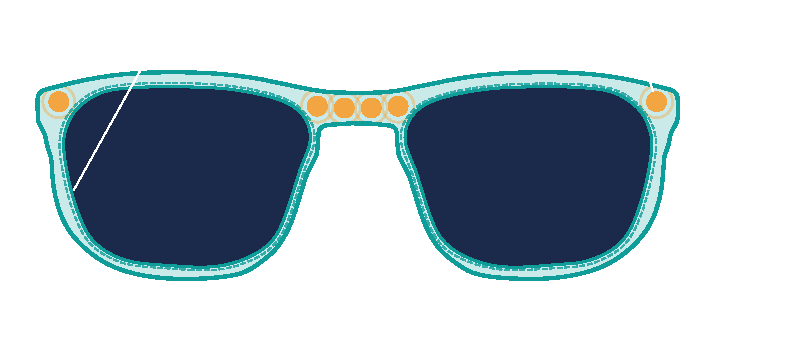
\includegraphics[width=16.5cm]{charts/cover_outline.pdf}};
  \node[anchor=north west,text width=17cm,white,align=left] at ($(current page.north west)+(2,-2.2)$)
    {{\sffamily\scriptsize\color{amber}TECHNICAL REPORT \textbullet{} PROMPT-ENGINEERING CASE STUDY \textbullet{} OCTOBER 2026}};
  \node[anchor=north west,text width=17.5cm,white,align=left] at ($(current page.center)+(-8.5,-1.6)$)
    {{\heavy\fontsize{34}{38}\selectfont Engineering a Magnetic\\3D-Cinema Clip-On with AI}\\[10pt]
     {\light\fontsize{15}{19}\selectfont From three phone photos and a hand-drawn curve to a\\print-ready, sub-millimetre part, by questioning every answer}};
  \node[anchor=south west,white,align=left] at ($(current page.south west)+(2,3.0)$)
    {{\sffamily\bfseries\large Balanagu Satya Siddhartha}\\[2pt]{\sffamily\small\color{grey} Design lead \& prompt engineer \textbullet{} AI agents in Blender, Python, Cura}};
  \node[anchor=south east,align=right] at ($(current page.south east)+(-2,3.0)$)
    {\begin{tabular}{@{}r@{\hspace{6pt}}l@{}}
     {\heavy\Large\color{amber}21} & {\sffamily\scriptsize\color{white}design versions}\\
     {\heavy\Large\color{amber}108} & {\sffamily\scriptsize\color{white}prompts}\\
     {\heavy\Large\color{amber}27} & {\sffamily\scriptsize\color{white}days}\\
     {\heavy\Large\color{amber}0.002} & {\sffamily\scriptsize\color{white}mm modelled median fit gap}\end{tabular}};
\end{tikzpicture}
\newpage

% =====================================================================  AT A GLANCE
\section*{At a glance}
\markboth{At a glance}{}
I wear prescription glasses with a thin steel frame. Passive 3D cinema glasses do not fit over them comfortably,
so I set out to build a 3.3-gram clip-on that holds the polarised film from cheap 3D glasses directly on my own frame, held by magnets.
I did not draw it in CAD. I \emph{directed AI agents} to build it in Blender through code, and I spent most of my effort on asking
the right questions, supplying real-world evidence, and refusing to accept confident answers that were not backed by a measurement.

\vspace{4pt}
\noindent\stat{3.26 g}{clip mass, PLA (4.90 g with\\ film and magnets)}{navy}\hfill
\stat{97.4\%}{of each model lens left clear\\(about 95.5\% of the photo-traced lens)}{teal}\hfill
\stat{0.002}{mm modelled median gap,\\clip to steel (p95 0.056)}{violet}\hfill
\stat{40$\times$}{estimated hold vs weight\\(1.9--2.7 N vs 0.048 N)}{coral}

\vspace{6pt}
\begin{center}
\begin{tikzpicture}[
  node distance=4mm and 5mm,
  src/.style={draw=navy!30,fill=mist,rounded corners=2pt,font=\sffamily\scriptsize,align=center,minimum width=2.45cm,minimum height=8mm},
  stage/.style={fill=navy,text=white,rounded corners=3pt,font=\sffamily\scriptsize\bfseries,align=center,minimum width=2.8cm,minimum height=11mm},
  gate/.style={draw=teal,fill=teal!10,rounded corners=2pt,font=\sffamily\scriptsize,align=center,minimum width=2.0cm,minimum height=7mm},
  outp/.style={fill=amber,text=navy,rounded corners=3pt,font=\sffamily\scriptsize\bfseries,align=center,minimum width=2.5cm,minimum height=9mm},
  ar/.style={-{Latex[length=2mm]},navy!60,line width=0.7pt}]
  % inputs
  \node[src] (p) {3 orthographic\\phone photos};
  \node[src,below=of p] (b) {hand-drawn outlines\\(front + B\'ezier top)};
  \node[src,below=of b] (s) {scale evidence: coin,\\6 mm grid, retailer sizes};
  \node[src,below=of s] (f) {film sheets + coin\\magnet spec (4$\times$1, 172 g)};
  % stages
  \node[stage,right=12mm of b] (m) {GLASSES MODEL\\\scriptsize\mdseries aligned $\to$ symmetric $\to$ $\times$1.011};
  \node[stage,below=8mm of m] (d) {CLIP DESIGN\\\scriptsize\mdseries outline, slot, lips, pockets};
  \foreach \n in {p,b} \draw[ar] (\n.east) -- (m.west);
  \foreach \n in {s} \draw[ar] (\n.east) -- ++(4mm,0) |- (m.west);
  \draw[ar] (f.east) -| ($(d.south west)+(4mm,0)$);
  \draw[ar] (m) -- (d);
  % gates
  \node[gate,right=14mm of m,yshift=8mm] (g1) {\faRuler\ shape \& size};
  \node[gate,below=2mm of g1] (g2) {\faCompress\ fit \& contact};
  \node[gate,below=2mm of g2] (g3) {\faMagnet\ magnets};
  \node[gate,below=2mm of g3] (g4) {\faHammer\ strength (FEA)};
  \node[gate,below=2mm of g4] (g5) {\faFilm\ film loading};
  \node[gate,below=2mm of g5] (g6) {\faEye\ view \& comfort};
  \node[gate,below=2mm of g6] (g7) {\faPrint\ printability};
  \node[draw=teal,dashed,rounded corners=4pt,fit=(g1)(g7),inner sep=2.5mm,label={[font=\sffamily\scriptsize\bfseries,text=teal]above:7 ANALYSIS GATES}] (G) {};
  \draw[ar] (d.east) -- (G.west|-d.east);
  \draw[ar,coral,dashed] (G.south) |- ++(0,-5mm) -| node[pos=0.25,below,font=\sffamily\tiny,text=coral]{any gate fails or I find a defect $\Rightarrow$ new version} (d.south);
  % outputs
  \node[outp,right=10mm of G,yshift=10mm] (o1) {STL + Cura 3mf\\+ UM2+ G-code};
  \node[outp,below=3mm of o1] (o2) {1:1 film cut\\template (PDF)};
  \node[outp,below=3mm of o2] (o3) {assembly \&\\dry-fit steps};
  \foreach \n in {o1,o2,o3} \draw[ar] (G.east) -- (\n.west);
\end{tikzpicture}
\end{center}
\captionof{figure}{The whole system on one page. Four kinds of real-world input feed a parametric glasses model and a clip design written as Python
for Blender; every version must pass seven analysis gates before any print file is written. A failed gate, or a defect I spotted, produced a new version.}

\begin{multicols}{2}\small
\textbf{\sffamily What this repository shows.}
\begin{itemize}
\item \textbf{Me}: how the idea started, how I framed the problem, how I questioned the AI and steered 21 versions to a final part.
\item \textbf{Method}: an evidence-first way of engineering a physical object with AI agents, with no CAD skills required.
\item \textbf{Playbook} (Part II): prerequisites, steps and copy-paste prompts so anyone can do the same for their glasses, including frames that are not magnetic.
\end{itemize}
\columnbreak
\textbf{\sffamily Honest status (27 Oct 2026).}
\begin{itemize}
\item Final design: \textbf{v15.1}, print files ready, sliced for an Ultimaker 2+ (2 h 9 min, 0.27 mm first layer then 0.1 mm).
\item Not yet verified on the real glasses: the dry fit and the real magnet pull. Section~\ref{sec:field} is reserved for the results once the part arrives.
\item Hold, strength and comfort numbers are model estimates, labelled as such.
\end{itemize}
\end{multicols}

\newpage
{\hypersetup{linkcolor=navy}\sffamily\tableofcontents}
\newpage

% =====================================================================  PART I
\clearpage\part{The engineer: how I approached it}

\Needspace{16\baselineskip}\section{The problem and how the idea started}
\Needspace{12\baselineskip}\subsection{The problem}
Cinemas hand out passive polarised 3D glasses. Worn over prescription glasses they slide, press on the nose, tilt the film away from the eye and
fog up. Commercial clip-on 3D lenses exist, but they are generic: they clip over the lens with sprung arms, cover part of the view and rarely match
a specific frame. I wanted something that disappears onto \emph{my} frame: same outline, no visible hardware, the full lens area used and
nothing touching my face.

\Needspace{12\baselineskip}\subsection{The first attempt that failed (and taught me the constraints)}
Before using AI at all, I tried a physical hack. I cut the two film sheets out of a pair of cinema 3D glasses, folded strips of aluminium from a
Coke can into hooks and glued them to the film so it could hang on my frame. The aluminium bent nicely, but the super glue \emph{spoiled the
film}. That failure gave me three hard constraints that shaped everything later:
\begin{enumerate}
\item The film is fragile: no cyanoacrylate (super glue) near it, since its fumes fog the polariser. Only 2-part epoxy, and only far from the film.
\item The film must stay flat: it can bow in one direction, never dome (I made this explicit to the AI in prompts 56 and 60).
\item The attachment must not rely on bending metal by hand; it must be repeatable and precise.
\end{enumerate}

\begin{prompt}{[11], 2 Oct}
the white red attachments on the filamnets are my experiment using coke tin cans so i can attach the filament directly on my glasses using
aluminium bending flexibility but its spoilling the filament when i use super glu to attach the attachments to the filament so i disgarded the project.
\end{prompt}

\Needspace{12\baselineskip}\subsection{The idea: let the frame itself be the fixture}
My glasses have a stainless-steel front. Steel is magnetic, so the frame can be the fixture: a thin printed carrier holds the film, and tiny
neodymium magnets in hidden pockets on its back snap onto the rims. Nothing touches the lens, nothing clamps, and it comes off with a peel.
I later \emph{tested} this assumption by sticking 20 loose magnets on the rims (13 Oct) to find where they hold and how many fit.

\begin{figure}[H]\centering
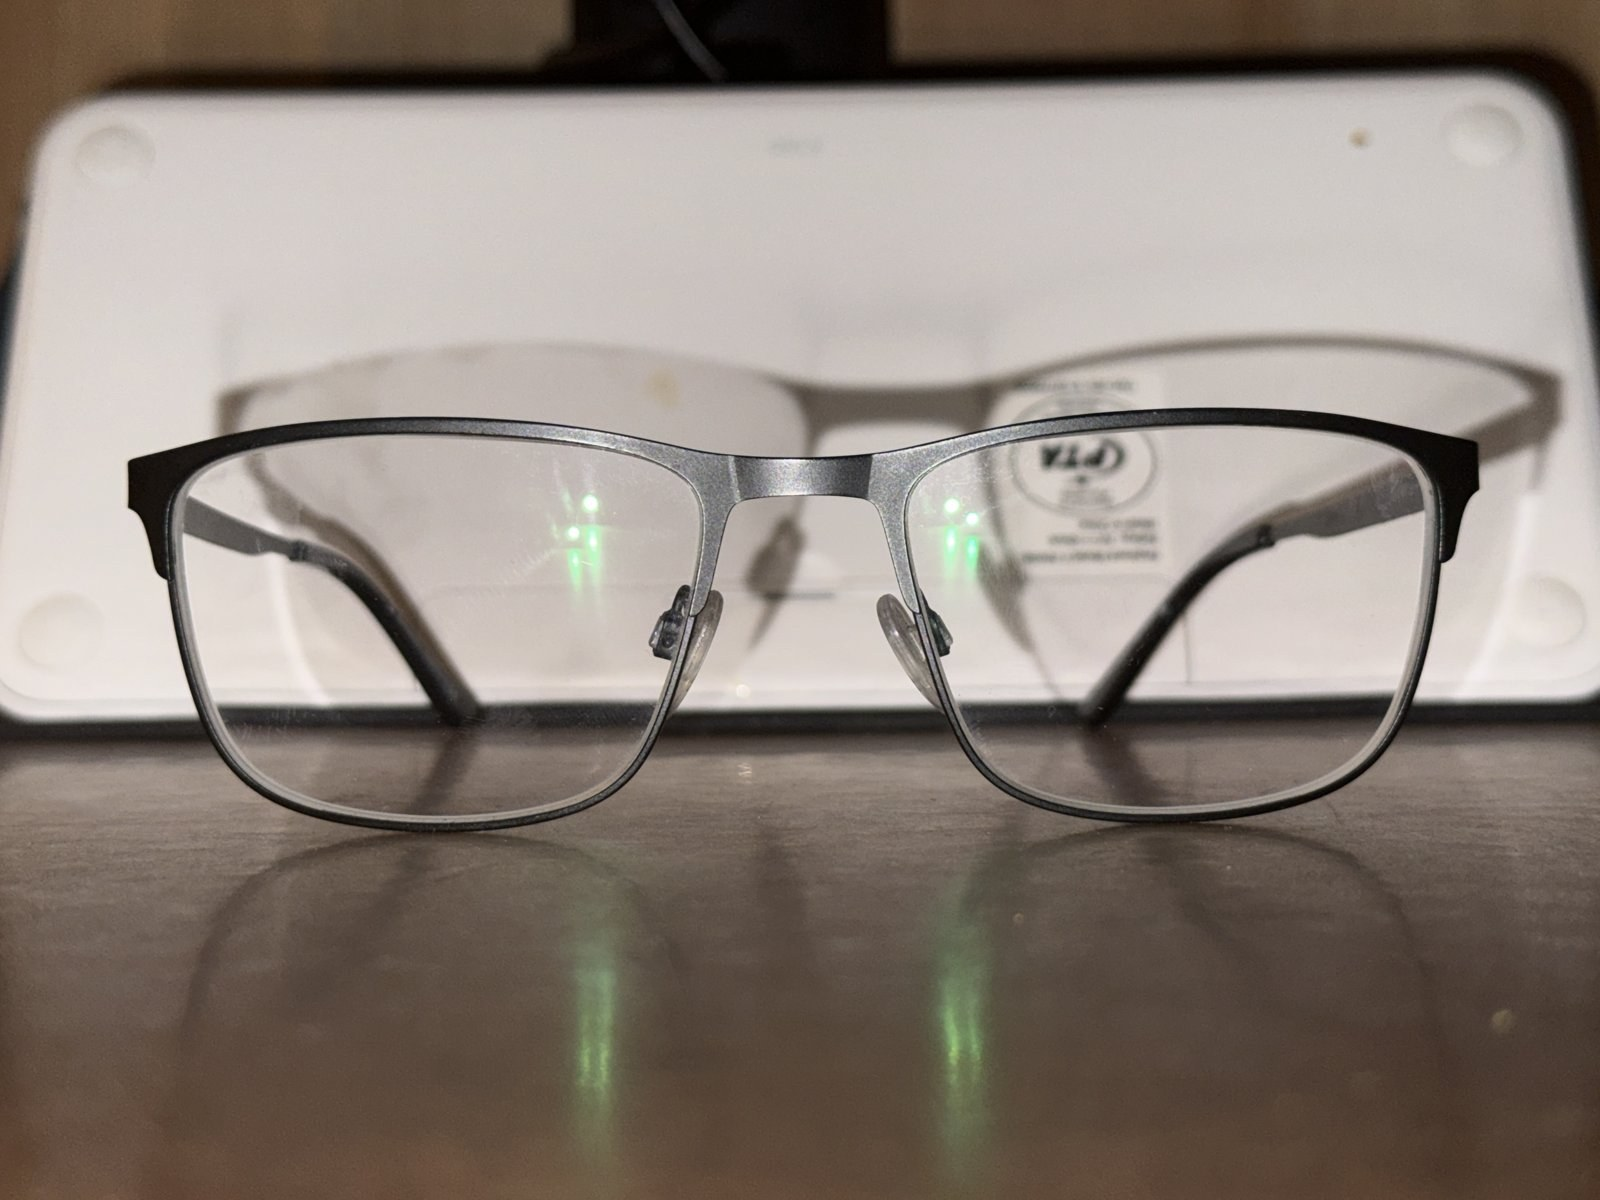
\includegraphics[height=3.3cm]{figures/photo_front.jpg}\hfill
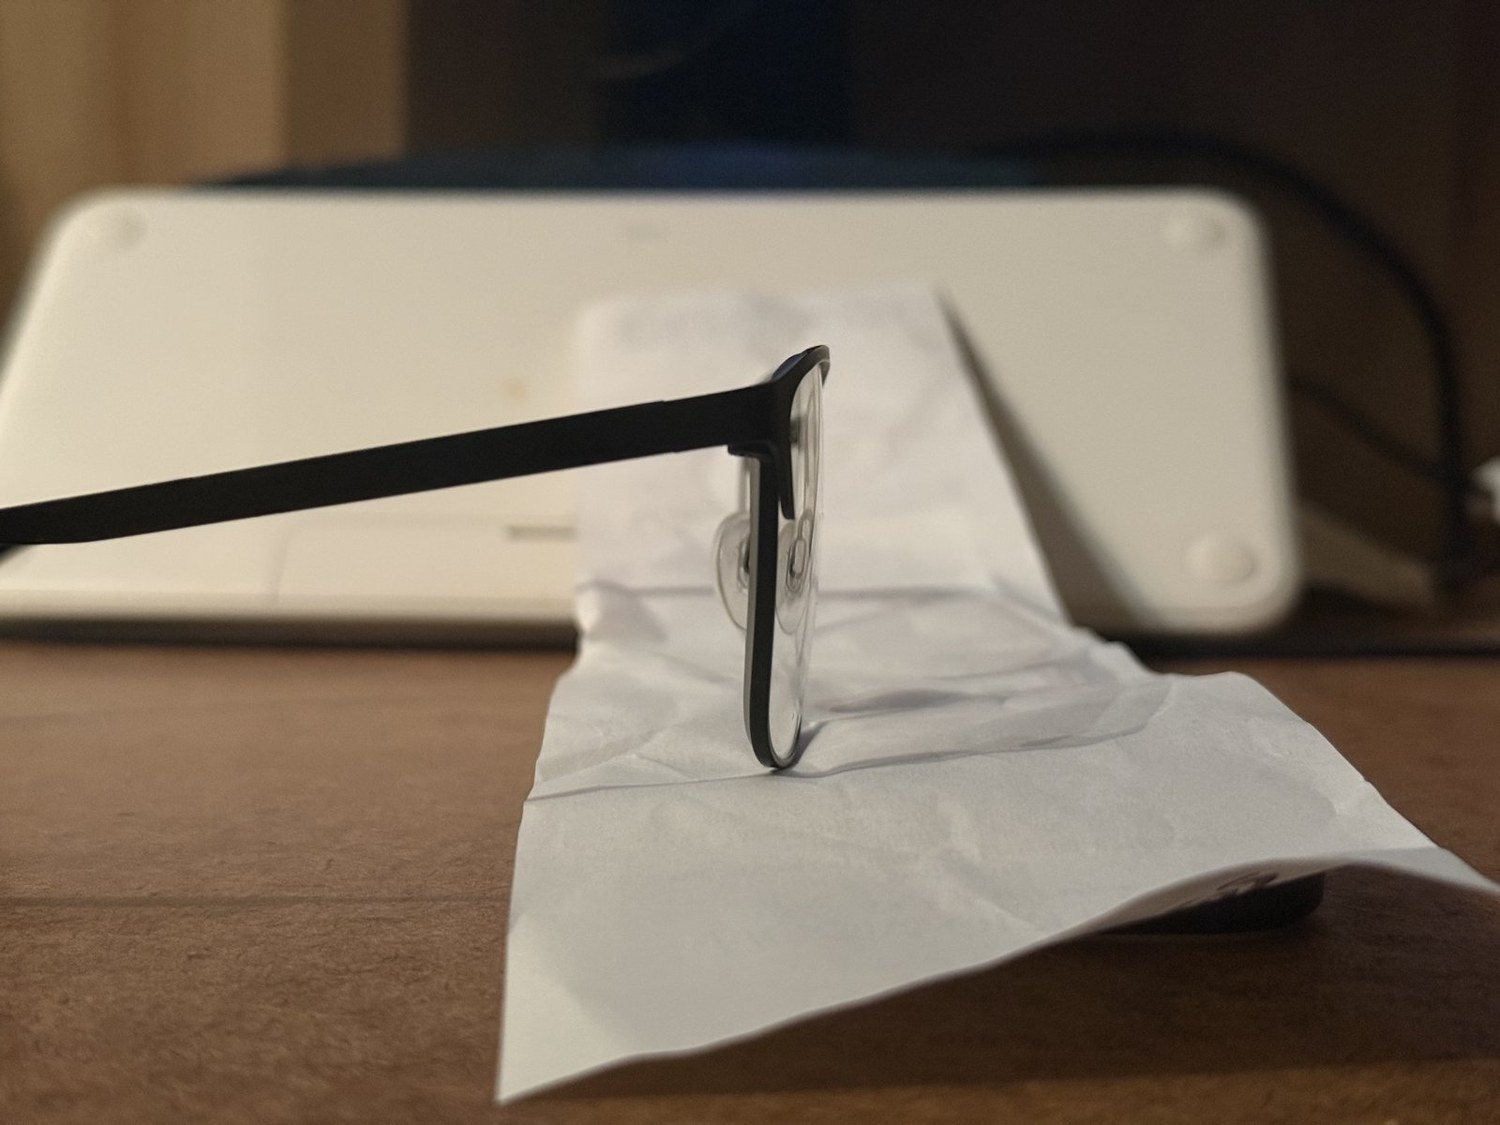
\includegraphics[height=3.3cm]{figures/photo_side.jpg}\hfill
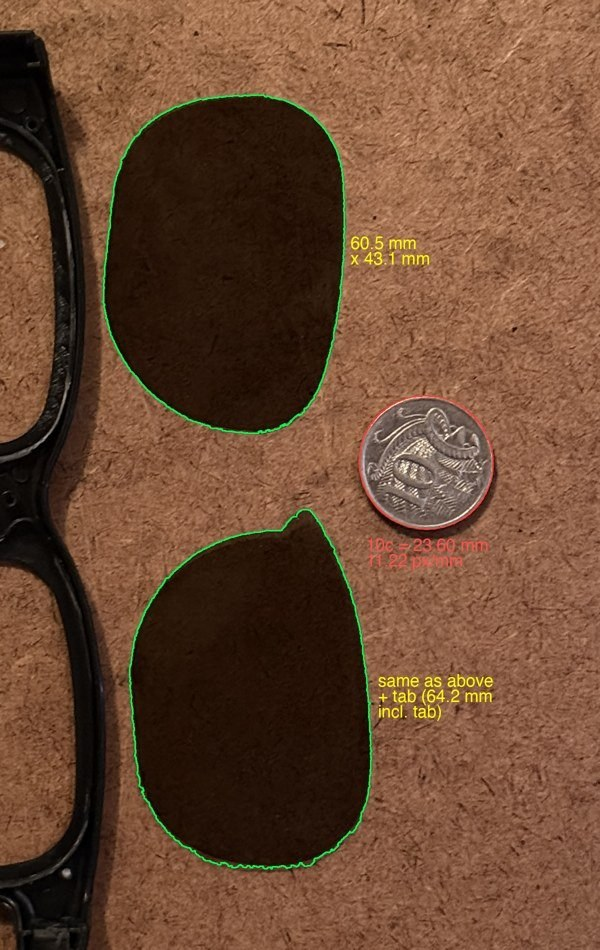
\includegraphics[height=3.3cm]{figures/photo_film_coin.jpg}
\caption{The only raw inputs at the start: three phone photos of my glasses (front, side, top not shown) and the two film sheets next to a 10-cent coin for scale.}
\end{figure}

\Needspace{16\baselineskip}\section{My approach: principles I set for the AI}
I treated the AI as a fast, tireless engineer who is \emph{overconfident} and occasionally forgets. My job was to set the rules of the game,
feed it ground truth and audit its claims. These principles emerged in the first days and I enforced them for the whole project.

\begin{center}
\begin{tikzpicture}[box/.style={rounded corners=4pt,fill=#1,text=white,minimum width=5.4cm,minimum height=2.45cm,text width=4.95cm,align=left,font=\sffamily\scriptsize,inner sep=6pt}]
\matrix[column sep=2mm,row sep=3mm]{
\node[box=navy]{{\bfseries\small\faPencil*\enspace Shape truth is mine}\\[2pt]The shape comes only from my hand-drawn outlines (front + B\'ezier top) and the side photo. Later photos may set \emph{size}, never shape.}; &
\node[box=teal]{{\bfseries\small\faBalanceScale\enspace Evidence over confidence}\\[2pt]``Are you sure?'' is a request for a number, a plot or a section view. A claim without a measurement is not accepted.}; &
\node[box=violet]{{\bfseries\small\faCrosshairs\enspace One-shot print mindset}\\[2pt]I have one chance to print. Every risk the analysis can see must be fixed before printing, not explained afterwards.}; \\
\node[box=coral]{{\bfseries\small\faRulerCombined\enspace Real world beats the model}\\[2pt]Coins, 6 mm grid paper, retailer sizes, the magnet datasheet and magnets stuck on the real rims override assumptions.}; &
\node[box=slate]{{\bfseries\small\faLayerGroup\enspace Never delete a variant}\\[2pt]Each version keeps its folder and report. Rejected ideas stay as evidence of why they failed.}; &
\node[box=amber!90!black]{{\bfseries\small\faUsers\enspace Many models, one owner}\\[2pt]One main model keeps the context; other models review or do bounded jobs. Their output is a claim, not a result.}; \\
};
\end{tikzpicture}
\end{center}

\Needspace{12\baselineskip}\subsection{Breaking the problem down}
Before any clip existed I insisted on a \emph{correct glasses model}, because every later number (contact, magnet seating, view) is measured against it.
The problem then decomposes into six coupled sub-problems. The difficulty is the coupling: moving a magnet changes the wall thickness, the
film slot, the clear view and the hold at the same time.

\begin{center}
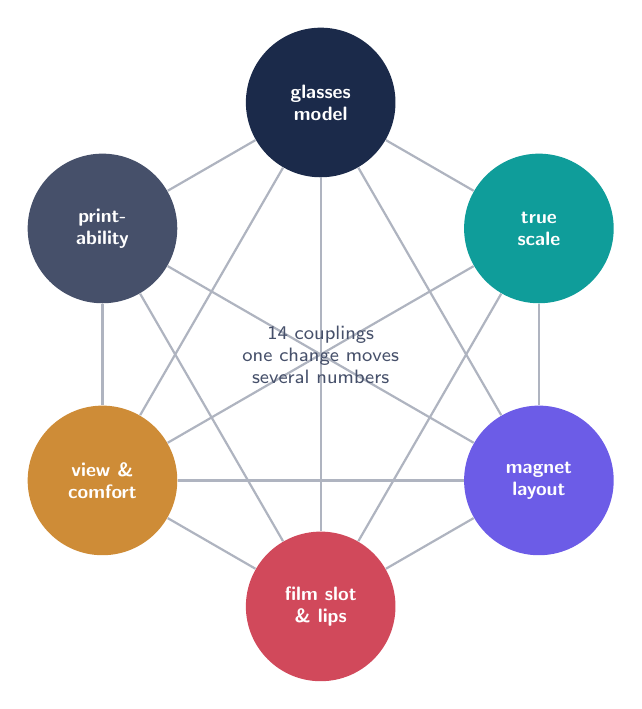
\begin{tikzpicture}[n/.style={circle,fill=#1,text=white,minimum size=19mm,font=\sffamily\scriptsize\bfseries,align=center},
  e/.style={navy!35,line width=0.8pt}]
  \node[n=navy] (a) at (90:3.2) {glasses\\model};
  \node[n=teal] (b) at (30:3.2) {true\\scale};
  \node[n=violet] (c) at (-30:3.2) {magnet\\layout};
  \node[n=coral] (d) at (-90:3.2) {film slot\\\& lips};
  \node[n=amber!85!black] (e) at (-150:3.2) {view \&\\comfort};
  \node[n=slate] (f) at (150:3.2) {print-\\ability};
  \foreach \x/\y in {a/b,a/c,a/d,a/e,b/c,b/d,c/d,c/e,d/e,d/f,e/f,f/a,c/f,b/e} \draw[e] (\x) -- (\y);
  \node[font=\sffamily\scriptsize,text=slate,align=center] at (0,0) {14 couplings\\one change moves\\several numbers};
\end{tikzpicture}
\end{center}

\Needspace{16\baselineskip}\section{The iteration journey}
The project ran from 1 to 27 October 2026. Figure~\ref{fig:timeline} shows every version, how long it lived and how many of my prompts
drove it. The large dot on \texttt{v00} is telling: about a third of the version-linked prompts went into the glasses model, not the clip.

\begin{figure}[H]\centering
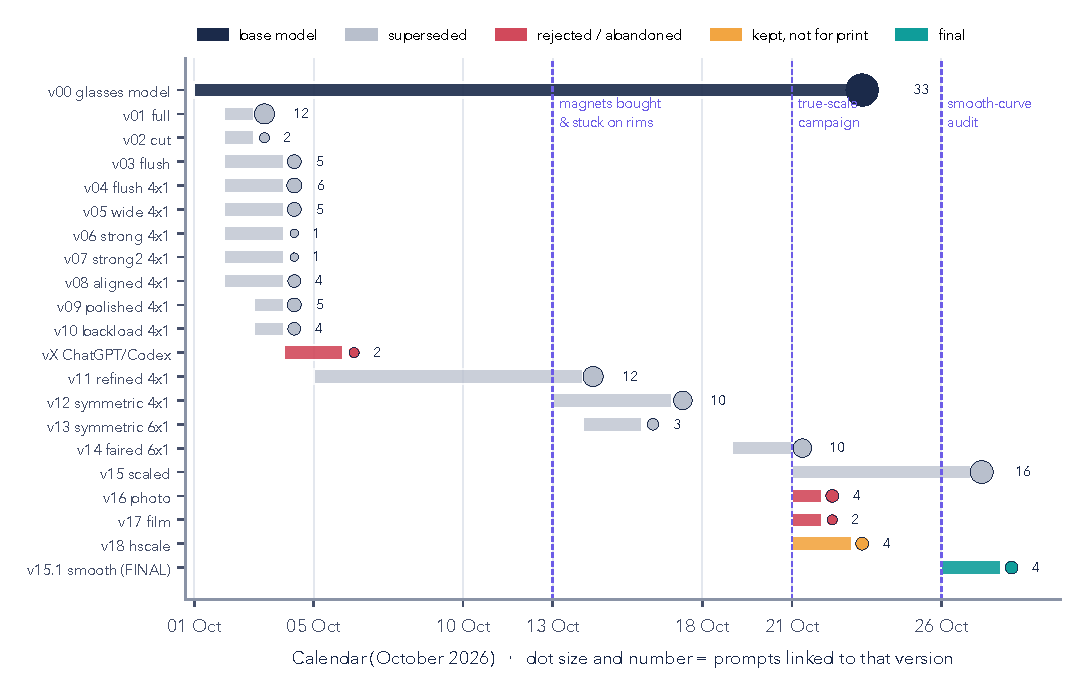
\includegraphics[width=\linewidth]{charts/version_timeline.pdf}
\caption{All 21 design versions on the calendar. Bars span first to last work; colour gives the final status. Purple lines mark the three turning points.}
\label{fig:timeline}
\end{figure}

\Needspace{12\baselineskip}\subsection{Seven phases}
\begin{center}
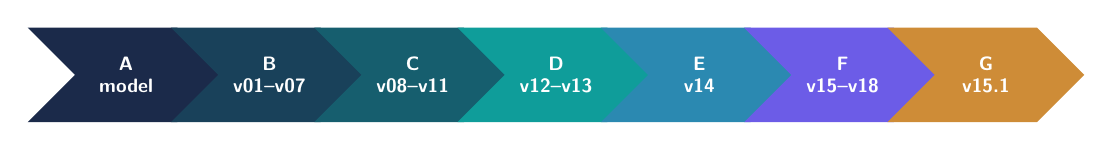
\begin{tikzpicture}[ph/.style={signal,signal to=east,signal from=west,fill=#1,text=white,minimum height=12mm,minimum width=2.5cm,font=\sffamily\scriptsize\bfseries,align=center,inner xsep=2pt}]
\node[ph=navy] (A) {A\\model};
\node[ph=navy!80!teal,right=-1mm of A] (B) {B\\v01--v07};
\node[ph=navy!55!teal,right=-1mm of B] (C) {C\\v08--v11};
\node[ph=teal,right=-1mm of C] (D) {D\\v12--v13};
\node[ph=teal!70!violet,right=-1mm of D] (E) {E\\v14};
\node[ph=violet,right=-1mm of E] (F) {F\\v15--v18};
\node[ph=amber!85!black,right=-1mm of F] (G) {G\\v15.1};
\end{tikzpicture}
\end{center}
\small
\begin{tabularx}{\linewidth}{@{}>{\sffamily\bfseries\color{teal}}l>{\raggedright\arraybackslash}p{3.4cm}X@{}}
\toprule
 & \sffamily\bfseries Phase & \sffamily\bfseries What happened and what I pushed for \\ \midrule
A & Glasses model (1--2 Oct) & Built from photos on three axes, not from the LiDAR scan. I told the AI my photos may be 1--2$^\circ$ off-axis and it may rotate them; I pushed alignment from ``about 80\%'' to tight. \\
B & First clips v01--v07 & Uncut film, cut film, flush outline, 4$\times$1 mm magnets (after I bought them), wider borders, magnets moved to spots I sketched. Nose collision drove most changes. \\
C & Aligned model v08--v11 & I spotted two spikes where the model drifted from my real centre piece $\Rightarrow$ rebuilt the model aligned first. Square magnet holes, smooth front, back-loaded film, film traced from the two real sheets. \\
D & Magnets v12--v13 & Datasheet pull is for 10 mm steel; on a vertical thin rim it drops to roughly 30\%. Mirror-symmetric frame. I stuck 20 magnets on the rims; six single magnets chosen. \\
E & Comfort \& print v14 & Multi-model review, nose-clearance and face-fit check from my photo, print orientation (upright, after I asked why not flat). \\
F & True scale v15--v18 & ``I only have one shot to print.'' Grid-paper and coin photos gave $\times$1.011. A photo-traced reshape (v16) broke my outline rule and was rejected; v18 ($\times$1.026 height) kept but not printed. \\
G & Smoothing v15.1 & I noticed the film cut was a wiggly trace, not a real constraint. Slot, lips and cut redrawn as smooth curves; all checks re-run. \\ \bottomrule
\end{tabularx}
\normalsize

\begin{figure}[H]\centering
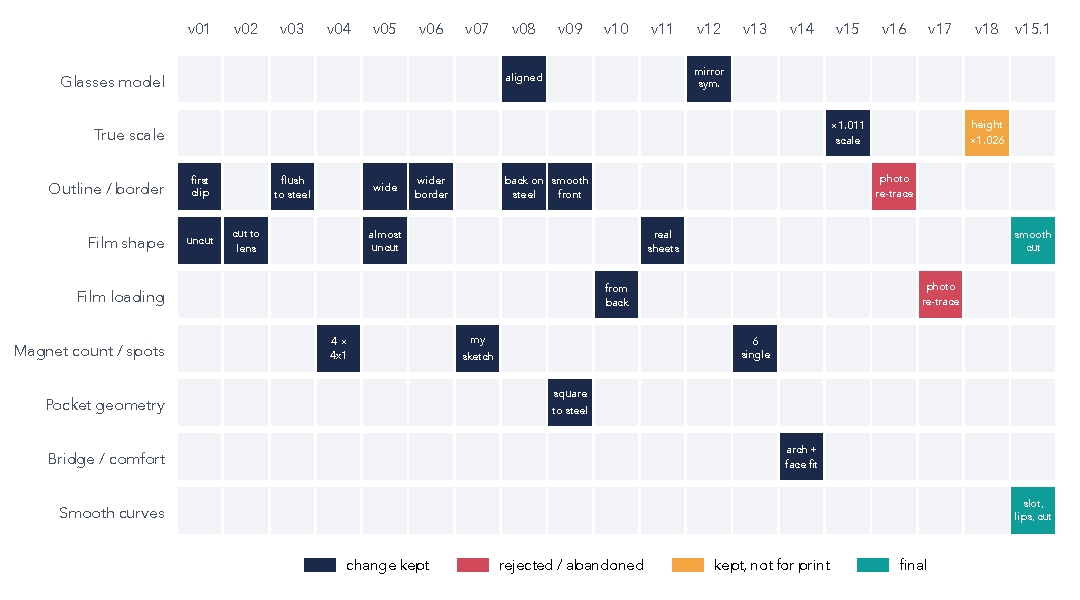
\includegraphics[width=\linewidth]{charts/version_changes.pdf}
\caption{What changed in each version. From the front the versions look almost identical; the engineering happened in tenths of a millimetre
in the attachment, fit, film slot and scale. Each coloured cell is a change and its trigger; Section~\ref{sec:verify} shows the checks behind them.}
\end{figure}

\Needspace{16\baselineskip}\section{How I questioned the AI}
\label{sec:question}
\Needspace{12\baselineskip}\subsection{The anatomy of my prompts}
I classified all 108 project prompts by intent (classification by a second model, checked by a script). Figure~\ref{fig:anatomy} shows when each
kind of prompt happened. Only one prompt stated the goal; \textbf{58 of 108 (54\%) were about checking rather than building}: 25 asked for a
verification, 17 corrected a specific defect and 16 challenged a claim. They cluster at the turning points (2--3 Oct, 21 Oct, 26 Oct): I usually
caught a problem first, then forced a new version.

\IfFileExists{charts/prompt_anatomy.pdf}{%
\begin{figure}[tbp]\centering
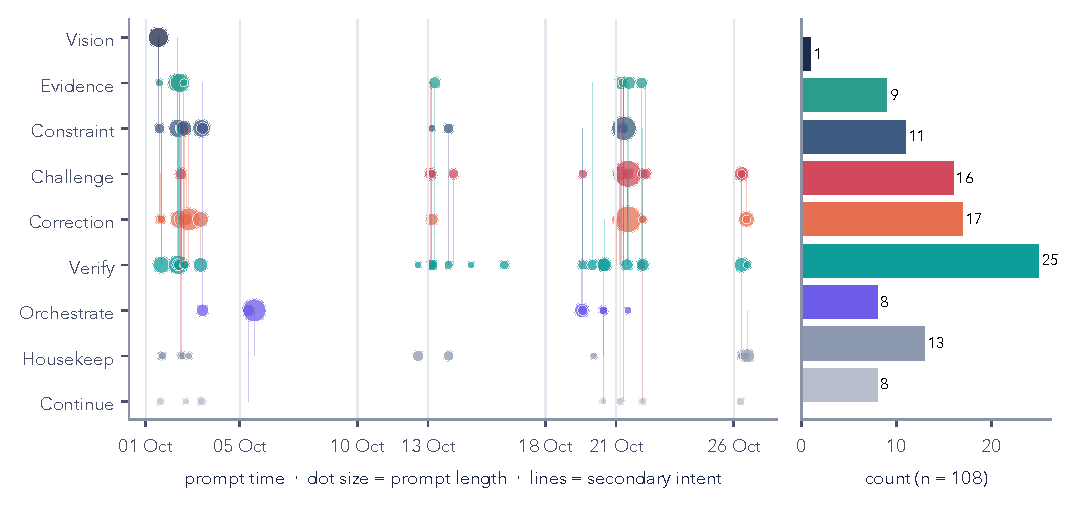
\includegraphics[width=\linewidth]{charts/prompt_anatomy.pdf}
\caption{Every prompt as a dot on the calendar, by primary intent; thin lines join a secondary intent. Right: totals.}
\label{fig:anatomy}
\end{figure}}{\begin{figure}[H]\centering\fbox{prompt anatomy chart pending}\caption{Prompt anatomy}\label{fig:anatomy}\end{figure}}

\Needspace{12\baselineskip}\subsection{The challenge loop}
Most of my progress came from one repeated loop. The AI made a confident claim; I asked for a visual or a number; I found what was wrong in it;
the finding became a permanent rule; the AI rebuilt; a gate checked the rule from then on.

\begin{center}
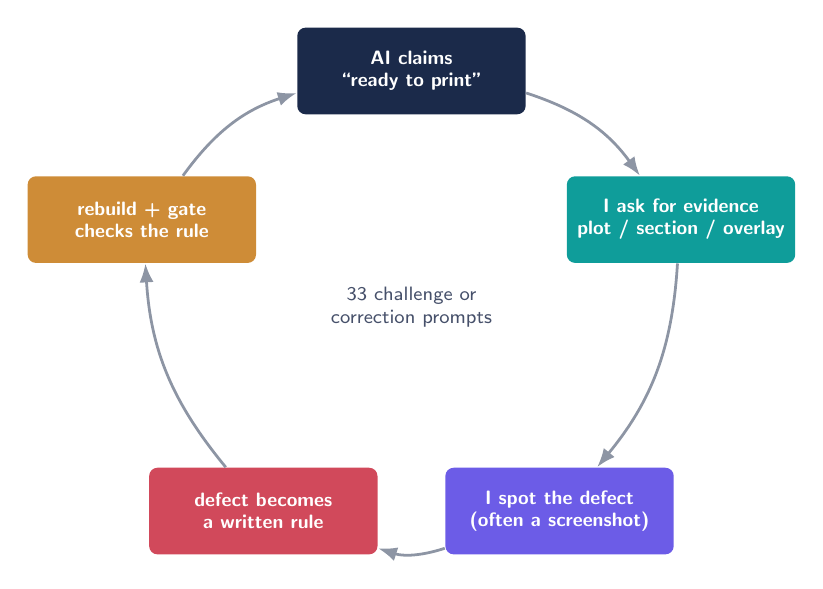
\begin{tikzpicture}[st/.style={rounded corners=3pt,fill=#1,text=white,font=\sffamily\scriptsize\bfseries,align=center,minimum width=2.9cm,minimum height=11mm},
  ar/.style={-{Latex[length=2.4mm]},line width=1pt,navy!50}]
  \node[st=navy] (1) at (90:3.0) {AI claims\\``ready to print''};
  \node[st=teal] (2) at (18:3.6) {I ask for evidence\\plot / section / overlay};
  \node[st=violet] (3) at (-54:3.2) {I spot the defect\\(often a screenshot)};
  \node[st=coral] (4) at (-126:3.2) {defect becomes\\a written rule};
  \node[st=amber!85!black] (5) at (162:3.6) {rebuild + gate\\checks the rule};
  \draw[ar] (1) to[bend left=18] (2); \draw[ar] (2) to[bend left=18] (3); \draw[ar] (3) to[bend left=18] (4);
  \draw[ar] (4) to[bend left=18] (5); \draw[ar] (5) to[bend left=18] (1);
  \node[font=\sffamily\scriptsize,text=slate,align=center] at (0,0) {33 challenge or\\correction prompts};
\end{tikzpicture}
\end{center}

\Needspace{20\baselineskip}\subsection{Case studies}
\Needspace{10\baselineskip}
\subsubsection{1. ``Why this gap?'': refusing a known defect}
\begin{minipage}[t]{0.56\linewidth}
\begin{prompt}{[44], 3 Oct}
why this gap? any reasoning ? you kept it even tho you know thats visible from your analysis ? you want to waste my time and tokens?
\end{prompt}
\begin{outcome}The AI's own contact analysis already showed the gap between clip back and steel. It had reported it instead of fixing it.
The clip back was rebuilt from the true steel surface (v08). Since then the rule is: never present a fit with a flaw the analysis shows.
Final v15.1: modelled median gap 0.002 mm.\end{outcome}
\end{minipage}\hfill
\begin{minipage}[t]{0.41\linewidth}\vspace{0pt}
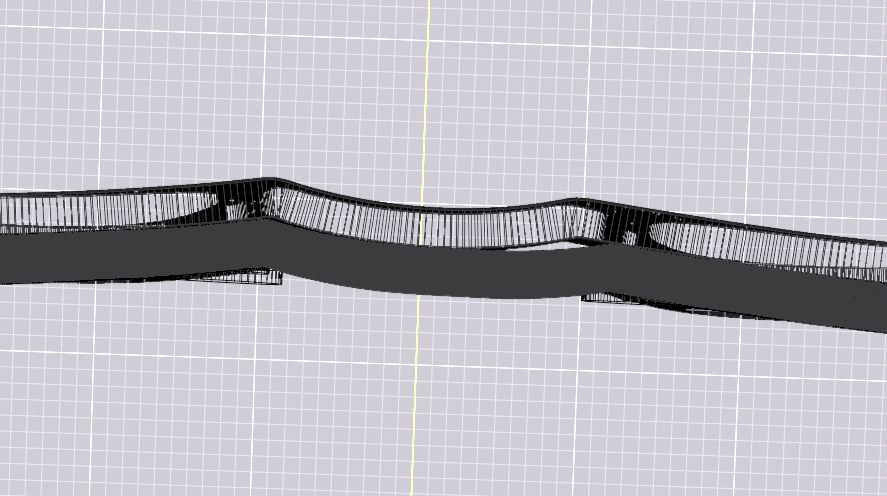
\includegraphics[width=\linewidth]{figures/markup_gap.jpg}\\[1pt]
{\sffamily\scriptsize\color{slate} My markup on the AI's render: the visible gap between clip and rim.}
\end{minipage}
\begin{figure}[H]\centering
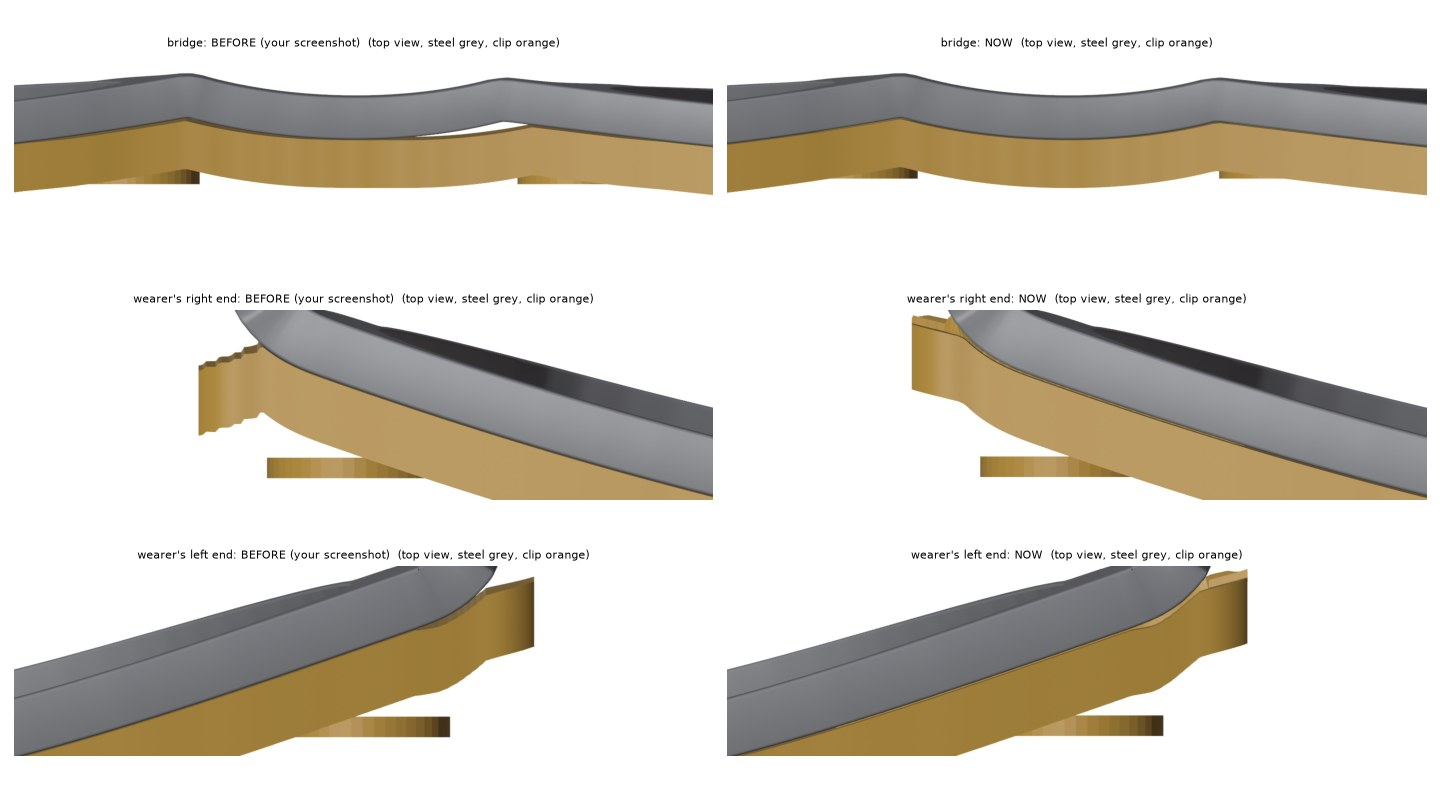
\includegraphics[width=\linewidth]{figures/gap_before_after.jpg}
\caption{The gap before and after the clip back was rebuilt from the true steel surface.}
\end{figure}

\Needspace{10\baselineskip}
\subsubsection{2. The slanted magnet hole and the hidden bevel}
\begin{minipage}[t]{0.56\linewidth}
\begin{prompt}{[48], 3 Oct}
the magnet hol is like slanty cylinder i dont think whats how a magnet hole should be ?? because when you place the magnet how will it rest
if thats the hole direction ... why are the holes visible from outside i want them covered only visible from the back
\end{prompt}
\begin{outcome}Pocket axes were tilted to the steel, so a magnet could not sit flat. Pockets were made square to the local steel surface,
blind from the front (cover $\ge$ 0.95 mm, final 1.183 mm), and the front got a gentle bevel I sketched to add thickness without blocking the view.\end{outcome}
\end{minipage}\hfill
\begin{minipage}[t]{0.41\linewidth}\vspace{0pt}
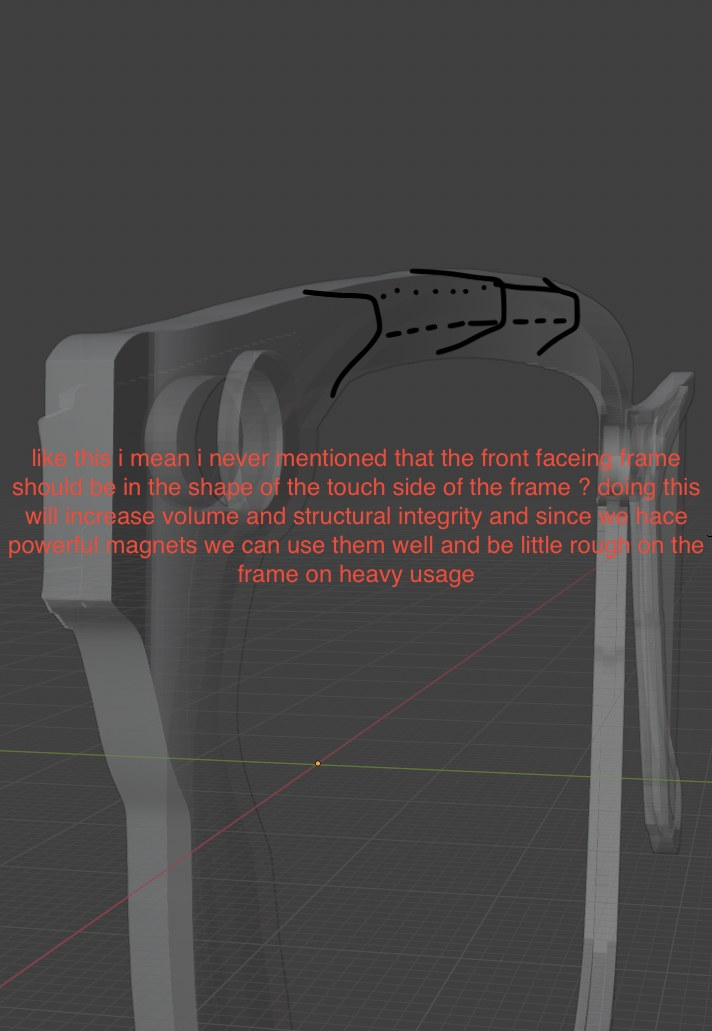
\includegraphics[width=\linewidth]{figures/markup_bevel.jpg}\\[1pt]
{\sffamily\scriptsize\color{slate} My sketched bevel profile on the AI's section.}
\end{minipage}
\begin{figure}[H]\centering
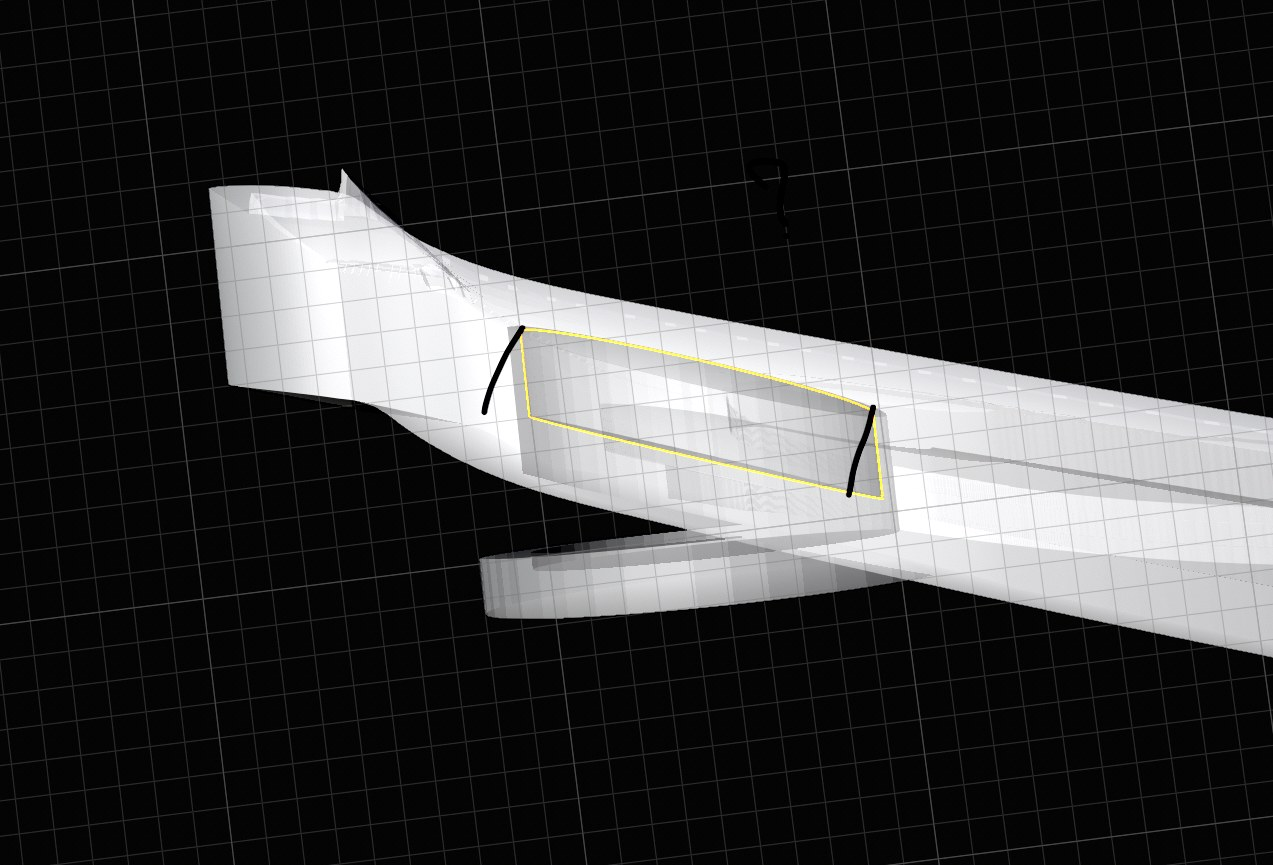
\includegraphics[width=0.8\linewidth]{figures/markup_hole.jpg}
\caption{My markup on the AI's render: the ``?'' on the slanted pocket that a magnet could not sit in flat.}
\end{figure}

\Needspace{10\baselineskip}
\subsubsection{3. Reading the datasheet more carefully than the AI}
\begin{prompt}{[72], 13 Oct}
are you sure? made sure all the parameters are considered and calculated? cause the magnets i bought felt not that strong but the manufacturer says its
``Pull Force: 0.172 kg'' [pasted the manufacturer's note: rated on 10 mm steel, about 30\% on a vertical surface, less on thin steel]
\end{prompt}
\begin{outcome}The hold model was re-derived with orientation, thin-steel saturation and air gap; I then asked to see where magnets can sit with a
depth/flatness map, stuck 20 magnets on my real rims to test, and asked for more magnets. Result: six single magnets (v13), 87--92\% of each magnet face over flat steel.\end{outcome}

\begin{figure}[tbp]\centering
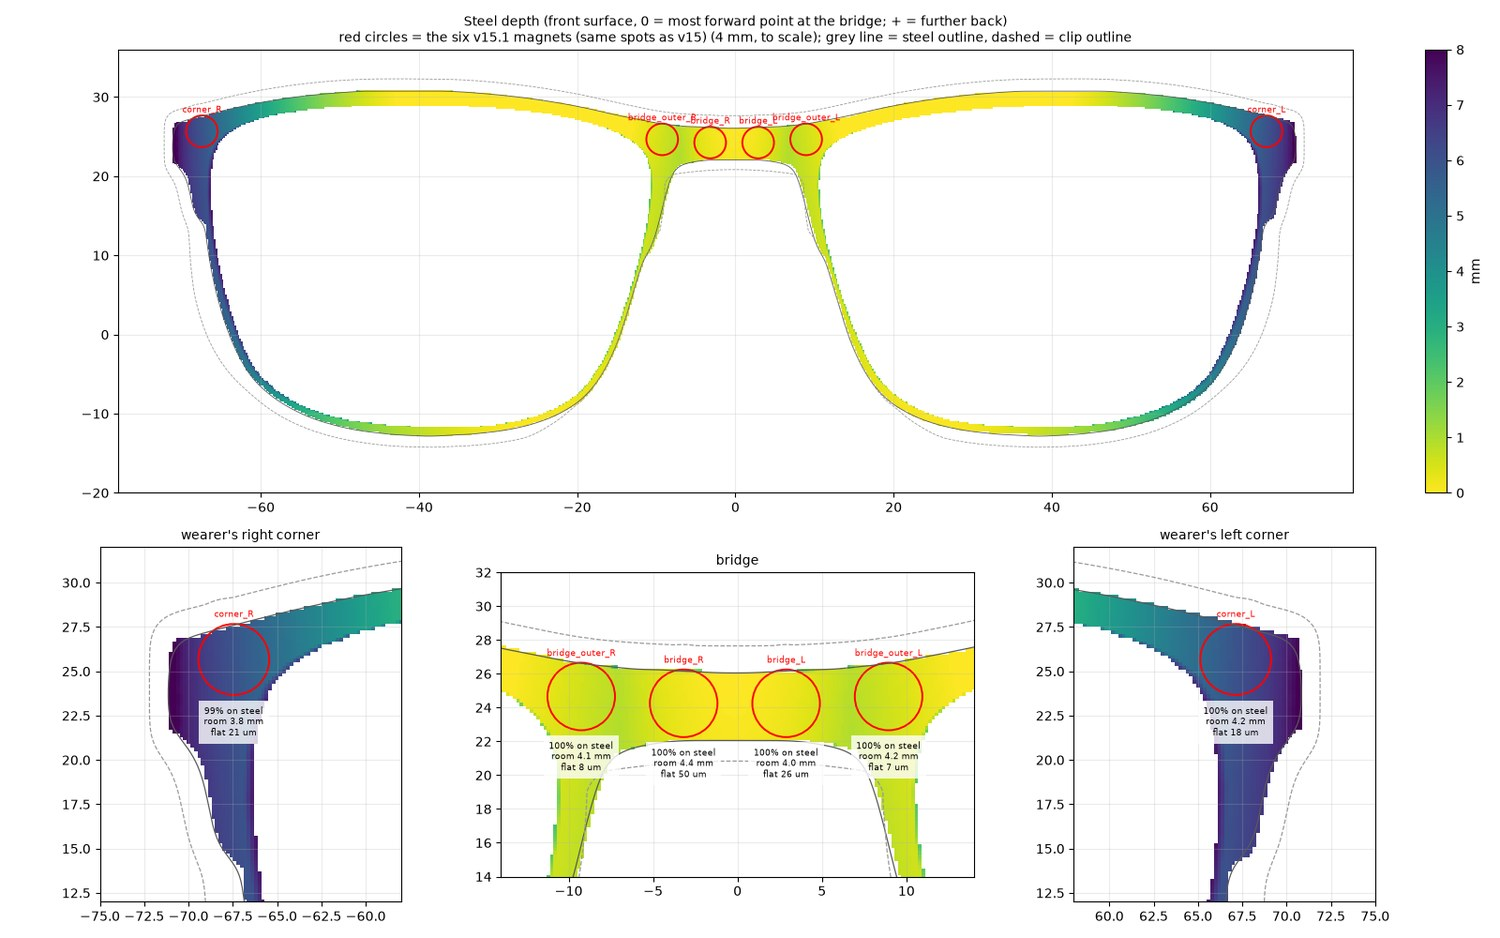
\includegraphics[width=0.56\linewidth]{figures/steel_depth.jpg}\\[4pt]
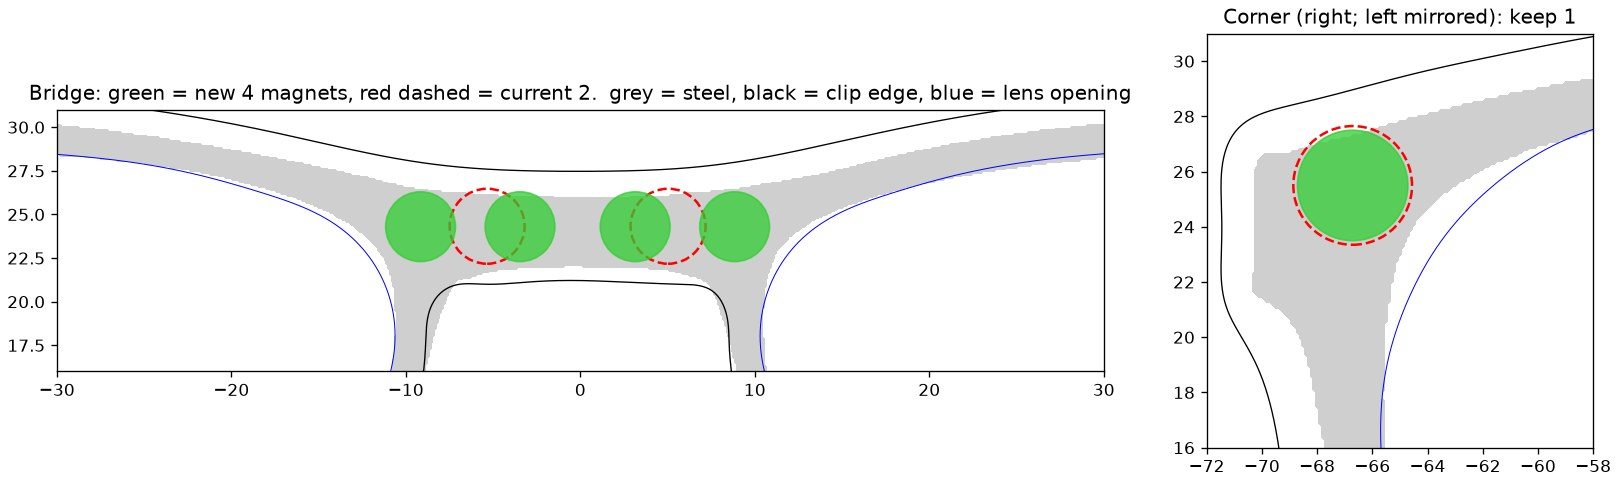
\includegraphics[width=0.88\linewidth]{figures/six_magnet_proposal.jpg}
\caption{Top: the steel depth and flatness map I asked for (prompt 86), so I could judge myself where a 4 mm magnet keeps contact. Bottom: the six-magnet proposal (green) against the old four (red dashed).}
\end{figure}

\Needspace{10\baselineskip}
\subsubsection{4. ``I only have one shot'': the true-scale campaign}
\begin{prompt}{[143] and [146], 21 Oct}
just wondering what are all the testing possibilities have you thought of and was so confident to send for printing cause i only have one shot to print
\ldots{} i gave the coins because they are well known you can look up in the internet to get exact measurement for more precision. i want this precision 2.345mm kindof
\end{prompt}
\begin{outcome}The model's absolute size had never been proven. I photographed the glasses on 6 mm grid paper with two cameras, a coin, a staple and a ruler.
Four independent sources were reconciled (Figure~\ref{fig:scale}); three agreed on $\times$1.011, which became v15. The one outlier was built as v18 and kept, not printed.\end{outcome}

\Needspace{10\baselineskip}
\subsubsection{5. Holding the AI to my outlines}
\begin{prompt}{[153], 21 Oct (strong language masked)}
you are allowed to take creative decisions but you should not be dumb at taking them right when I \ldots{} manually slogged my a** drawing those outlines for you,
how come you f*** it up again? \ldots{} You're not actually fact checking
\end{prompt}
\begin{outcome}v16 had silently reshaped the clip from a photo re-trace, against my rule that shape comes only from my outlines. It was rejected, a full audit of all versions
was run, and the rule was written into every later brief.\end{outcome}

\Needspace{10\baselineskip}
\subsubsection{6. The wiggly film cut}
\begin{prompt}{[174], 26 Oct}
look at this film cut i thought you are cropping it because it is causing issues with the magnet placement but looking at the blend file this purly your incapacity to draw simple
outline around a film and because of that now the user (me) should suffer cutting the film in this complex shape to fit properly.
\end{prompt}
\begin{outcome}The slot, lips and cut line followed a noisy photo trace (0.1--1 mm wiggles). They were redrawn as smooth curves (v15.1) and every check was re-run.
New rule: anything a person cuts by hand must be smooth; odd shapes must be explained up front.\end{outcome}

\Needspace{16\baselineskip}\section{Engineering with AI: orchestration}
\Needspace{12\baselineskip}\subsection{The setup}
I ran the project with one \emph{main} model that kept the full context and wrote the Blender/Python code, plus other models for bounded jobs and
independent reviews, coordinated by my own orchestration console (Agent Hub). Workers had no Blender in their sandbox, so geometry builds stayed
with the main model while analysis scripts, documentation and reviews were delegated.

\begin{center}
\begin{tikzpicture}[
  me/.style={circle,fill=amber,text=navy,minimum size=20mm,font=\sffamily\scriptsize\bfseries,align=center},
  main/.style={rounded corners=4pt,fill=navy,text=white,minimum width=4.2cm,minimum height=14mm,font=\sffamily\scriptsize\bfseries,align=center},
  w/.style={rounded corners=3pt,draw=#1,fill=#1!8,minimum width=3.3cm,minimum height=10mm,font=\sffamily\scriptsize,align=center},
  t/.style={rounded corners=3pt,fill=mist,minimum width=3.3cm,minimum height=9mm,font=\sffamily\scriptsize,align=center},
  ar/.style={-{Latex[length=2mm]},line width=0.8pt,navy!55}]
  \node[me] (me) {ME\\goals, rules,\\evidence};
  \node[main,right=14mm of me] (m) {MAIN MODEL\\\mdseries keeps context, plans,\\writes Blender Python, accepts};
  \node[w=teal,right=16mm of m,yshift=14mm] (w1) {implementer workers\\\tiny analysis scripts, docs};
  \node[w=violet,right=16mm of m] (w2) {independent reviewers\\\tiny one ``lens'' each};
  \node[w=coral,right=16mm of m,yshift=-14mm] (w3) {side attempt (ChatGPT)\\\tiny rejected, mined for ideas};
  \node[t,below=12mm of m,xshift=-22mm] (b) {\faCube\ Blender 4.3 (headless)\\\tiny clip + glasses scenes};
  \node[t,right=4mm of b] (py) {\faPython\ numpy / scipy / shapely\\\tiny FEA, contact, film sweep};
  \node[t,right=4mm of py] (cu) {\faPrint\ CuraEngine\\\tiny slicing, G-code};
  \node[t,right=4mm of cu] (g) {\faShield*\ gate.sh\\\tiny thresholds + hashes};
  \draw[ar] (me) -- node[above,font=\sffamily\tiny]{prompts} (m);
  \draw[ar] (m.south) -- ++(0,-5mm) -| (b.north); \draw[ar] (m.south) -- ++(0,-5mm) -| (py.north);
  \draw[ar] (m.south) -- ++(0,-5mm) -| (cu.north); \draw[ar] (m.south) -- ++(0,-5mm) -| (g.north);
  \foreach \n in {w1,w2} {\draw[ar] (m.east) -- (\n.west); }
  \draw[ar,coral,dashed] (w3.west) -- (m.east);
  \draw[ar,teal,dashed] (m.north) to[bend right=25] node[above,font=\sffamily\tiny]{evidence: plots, sections, numbers} (me.north);
\end{tikzpicture}
\end{center}

\Needspace{12\baselineskip}\subsection{What I did differently}
\begin{itemize}
\item \textbf{Reviews with lenses.} For v13 I asked for the 3D model and my full request history to be given to several models, each asked to find issues
through one lens (``making and using the real part'', smoothness, accuracy), backed by numbers or file lines. The main model then verified each finding before changing anything (prompt 108).
\item \textbf{Workers are claims, not results.} Worker output counted only after a check script passed and the diff was read. One worker's note said outputs were
missing when they existed; it was caught because results were re-derived from the source.
\item \textbf{Budget-aware delegation.} I explicitly steered usage (``use agents hub to minimise the load'', ``use GPT 6.1, it's literally free''), and
also limited it: no other model edits the main work unless I say so (prompt 111).
\item \textbf{Cross-model comparison.} When the ChatGPT side attempt came back (4--5 Oct) I rejected it, then had the main model read its prompts and outputs and improve on them.
Its numbers (e.g. 99.8\% clear view) relied on a fictional oversized film contour, a good example of a confident but wrong result.
\item \textbf{Everything reproducible.} Each version has a build chain (\texttt{chain.sh}), a gate (\texttt{gate.sh}) with numeric thresholds and SHA-256 checks
that the protected glasses models are untouched, a report, and my linked prompts.
\end{itemize}

\Needspace{16\baselineskip}\section{Verification: seven gates}
\label{sec:verify}
Every number below is for the final v15.1 unless noted. Figure~\ref{fig:margins} puts the critical ones against their thresholds.

\begin{figure}[H]\centering
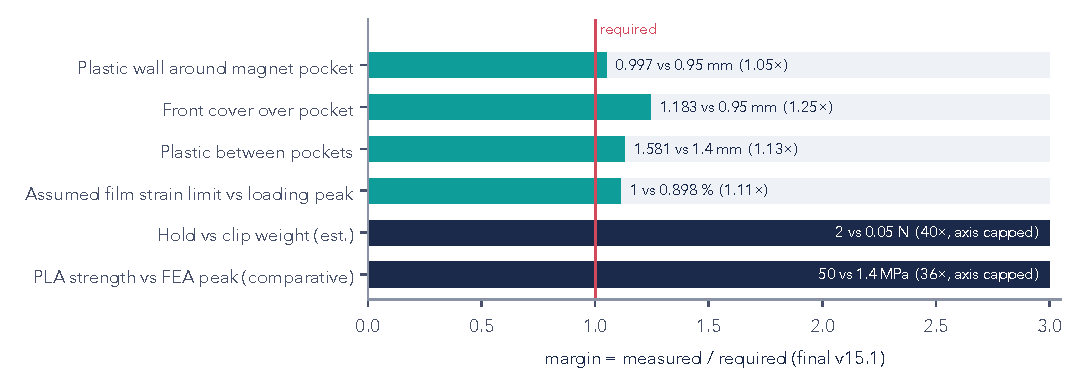
\includegraphics[width=\linewidth]{charts/margins.pdf}
\caption{Margins of the final design. Thin-wall margins are deliberately small: every 0.1 mm of plastic is 0.1 mm of lost view. Hold and strength numbers are estimates (comparative FEA, typical PLA strength 50 MPa).}
\label{fig:margins}
\end{figure}

\begin{figure}[H]\centering
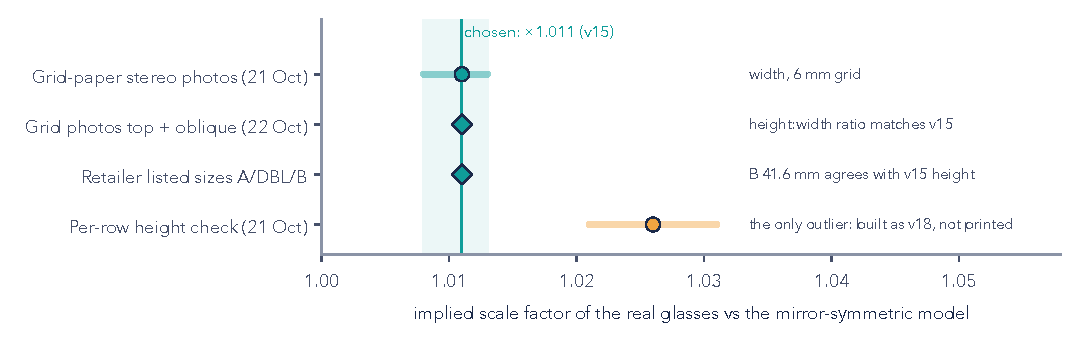
\includegraphics[width=\linewidth]{charts/scale_evidence.pdf}
\caption{True scale. Four independent sources; three agree on $\times$1.011. The per-row height check is the outlier, so its variant (v18) is kept for reference only.}
\label{fig:scale}
\end{figure}

\Needspace{12\baselineskip}\subsection{Gate 1 -- Shape and size}
\begin{figure}[H]\centering
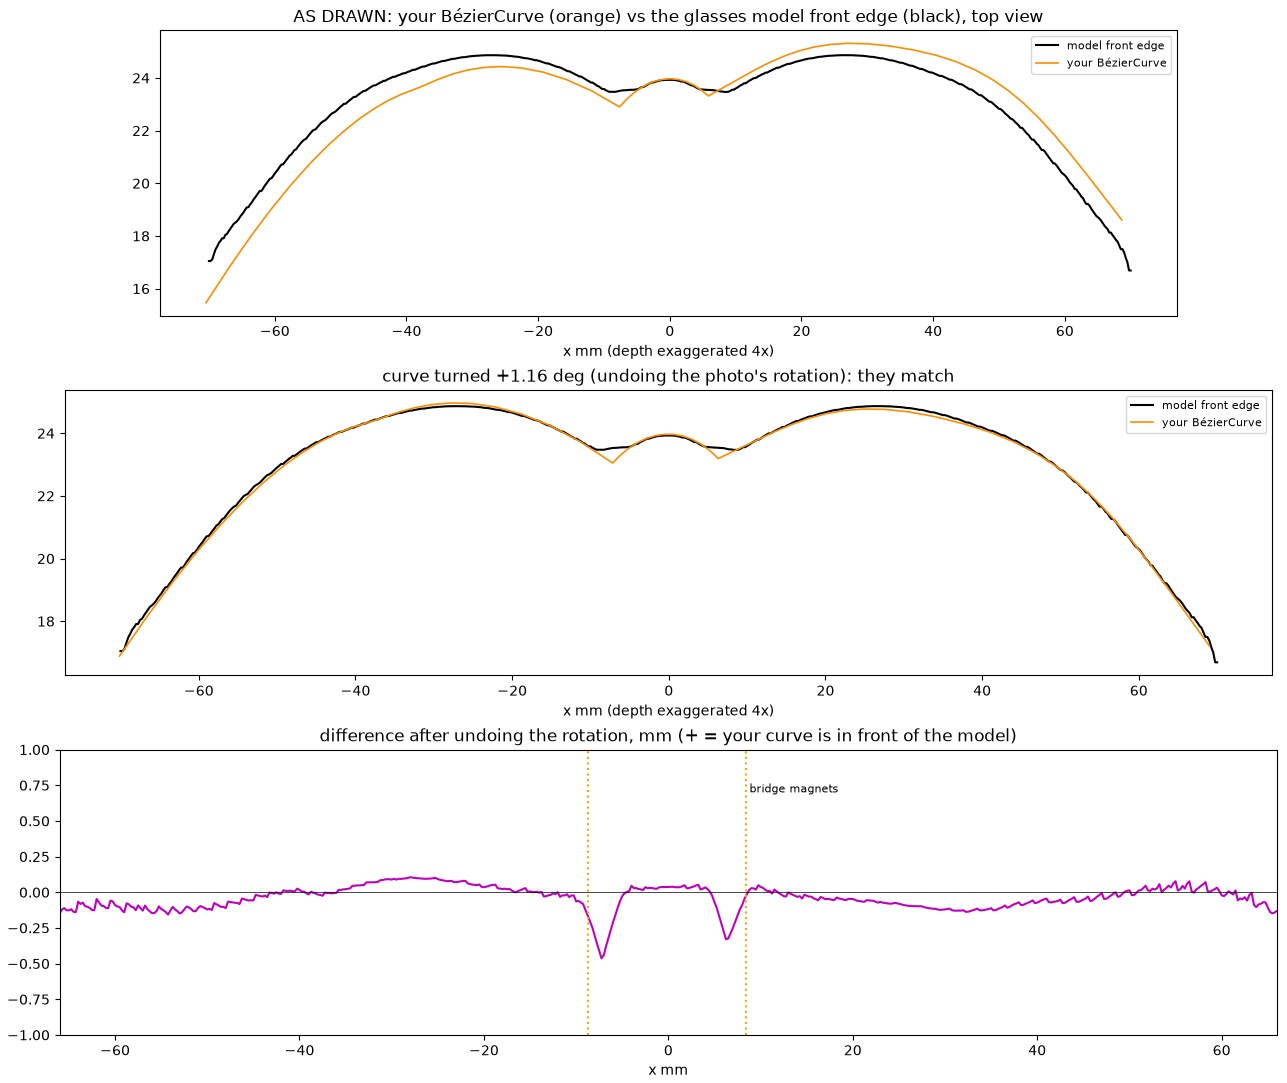
\includegraphics[height=5.78cm]{figures/model_vs_bezier.jpg}\hfill
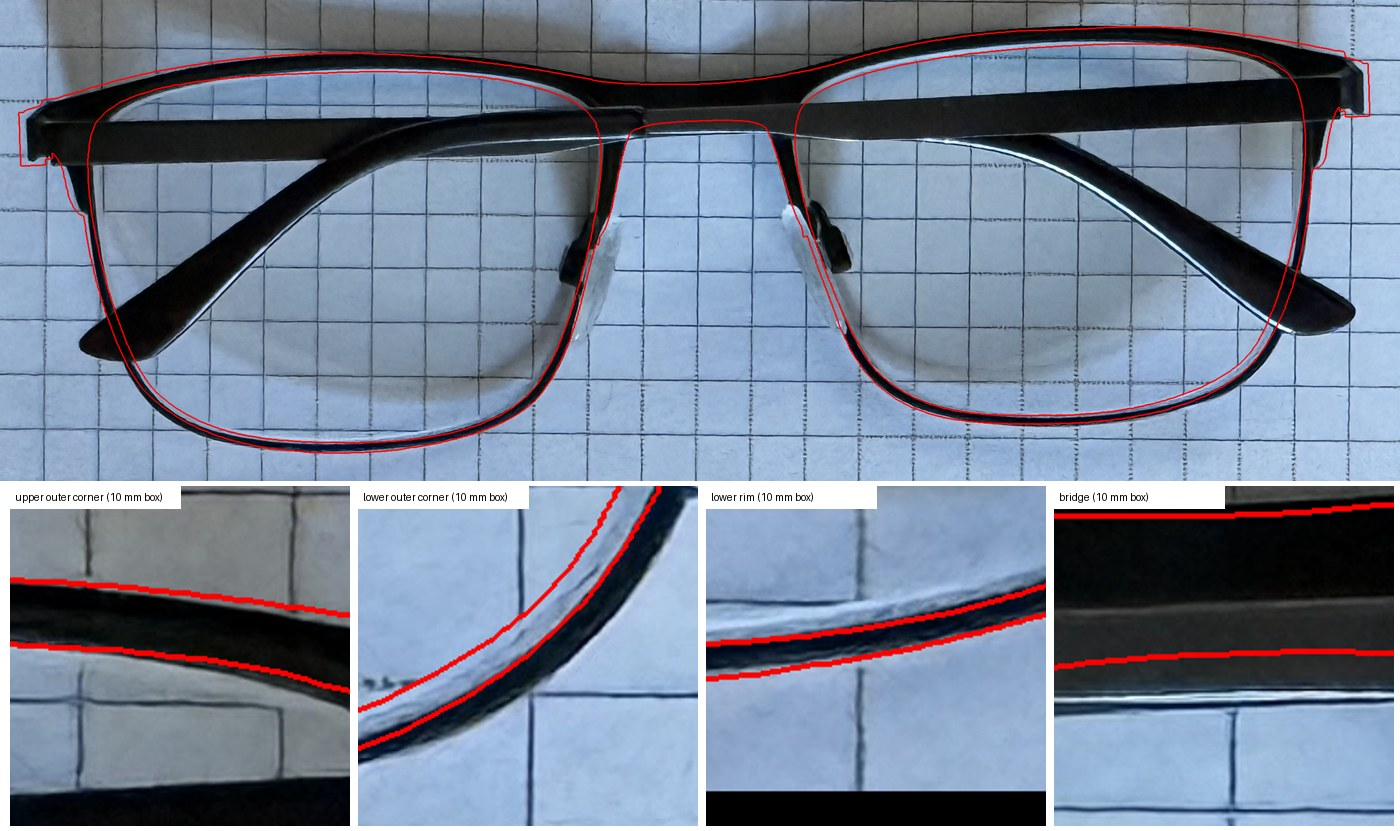
\includegraphics[height=5.78cm]{figures/grid_fit.jpg}
\caption{Left: model top view against my hand-drawn B\'ezier curve. Right: model outline fitted to the glasses photographed on 6 mm grid paper.}
\end{figure}

\Needspace{12\baselineskip}\subsection{Gate 2 -- Fit and contact}
\begin{figure}[H]\centering
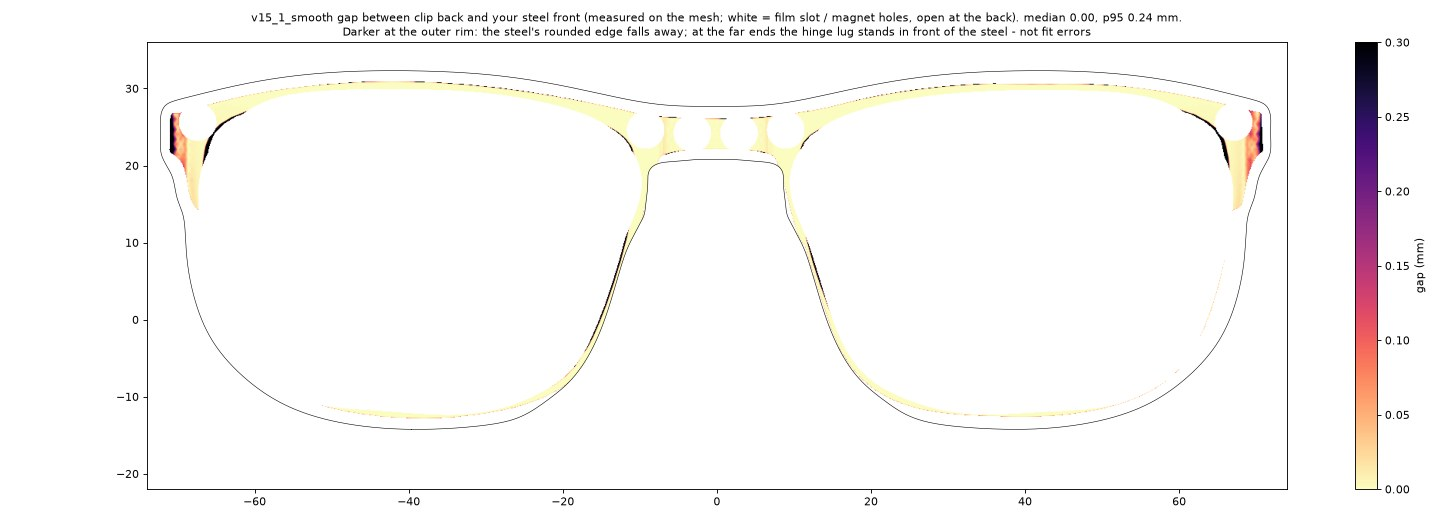
\includegraphics[width=\linewidth]{figures/gap.jpg}
\caption{Modelled gap from the clip back to the steel model. Median 0.002 mm, 95th percentile 0.056 mm. The real gap is measured at the dry fit.}
\end{figure}

\Needspace{12\baselineskip}\subsection{Gate 3 -- Magnets}
\begin{figure}[H]\centering
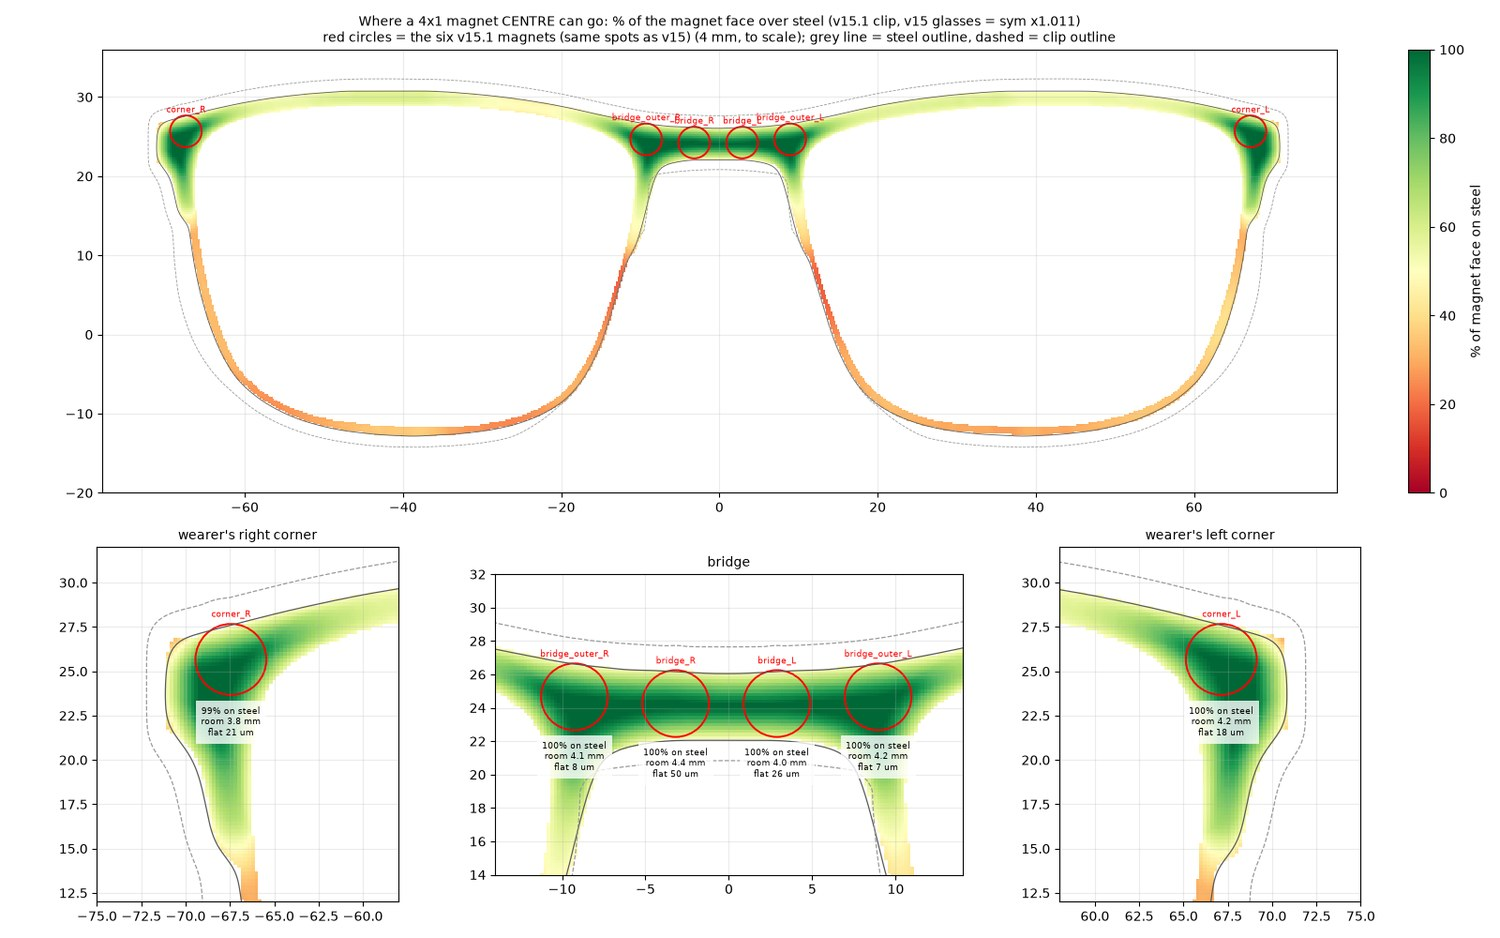
\includegraphics[height=5.06cm]{figures/magnet_spots.jpg}\hfill
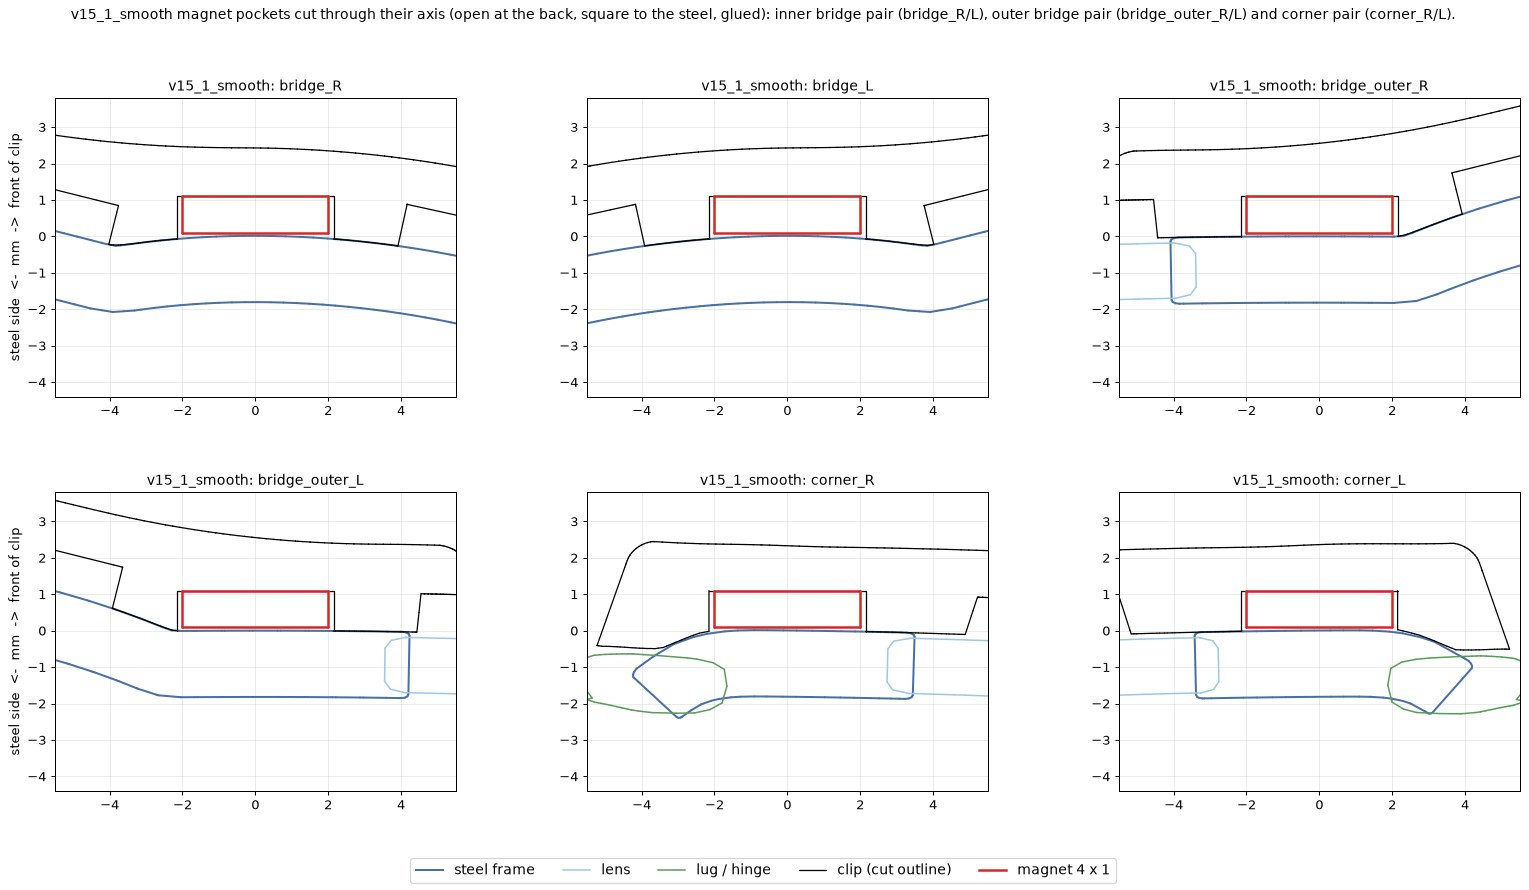
\includegraphics[height=5.06cm]{figures/pockets.jpg}
\caption{Six pockets: four at the bridge, two at the outer corners. Right: sections through each pocket; magnet face 0.08--0.16 mm from the steel, wall $\ge$ 0.997 mm, front cover $\ge$ 1.183 mm.}
\end{figure}

\Needspace{12\baselineskip}\subsection{Gate 4 -- Strength}
\begin{figure}[H]\centering
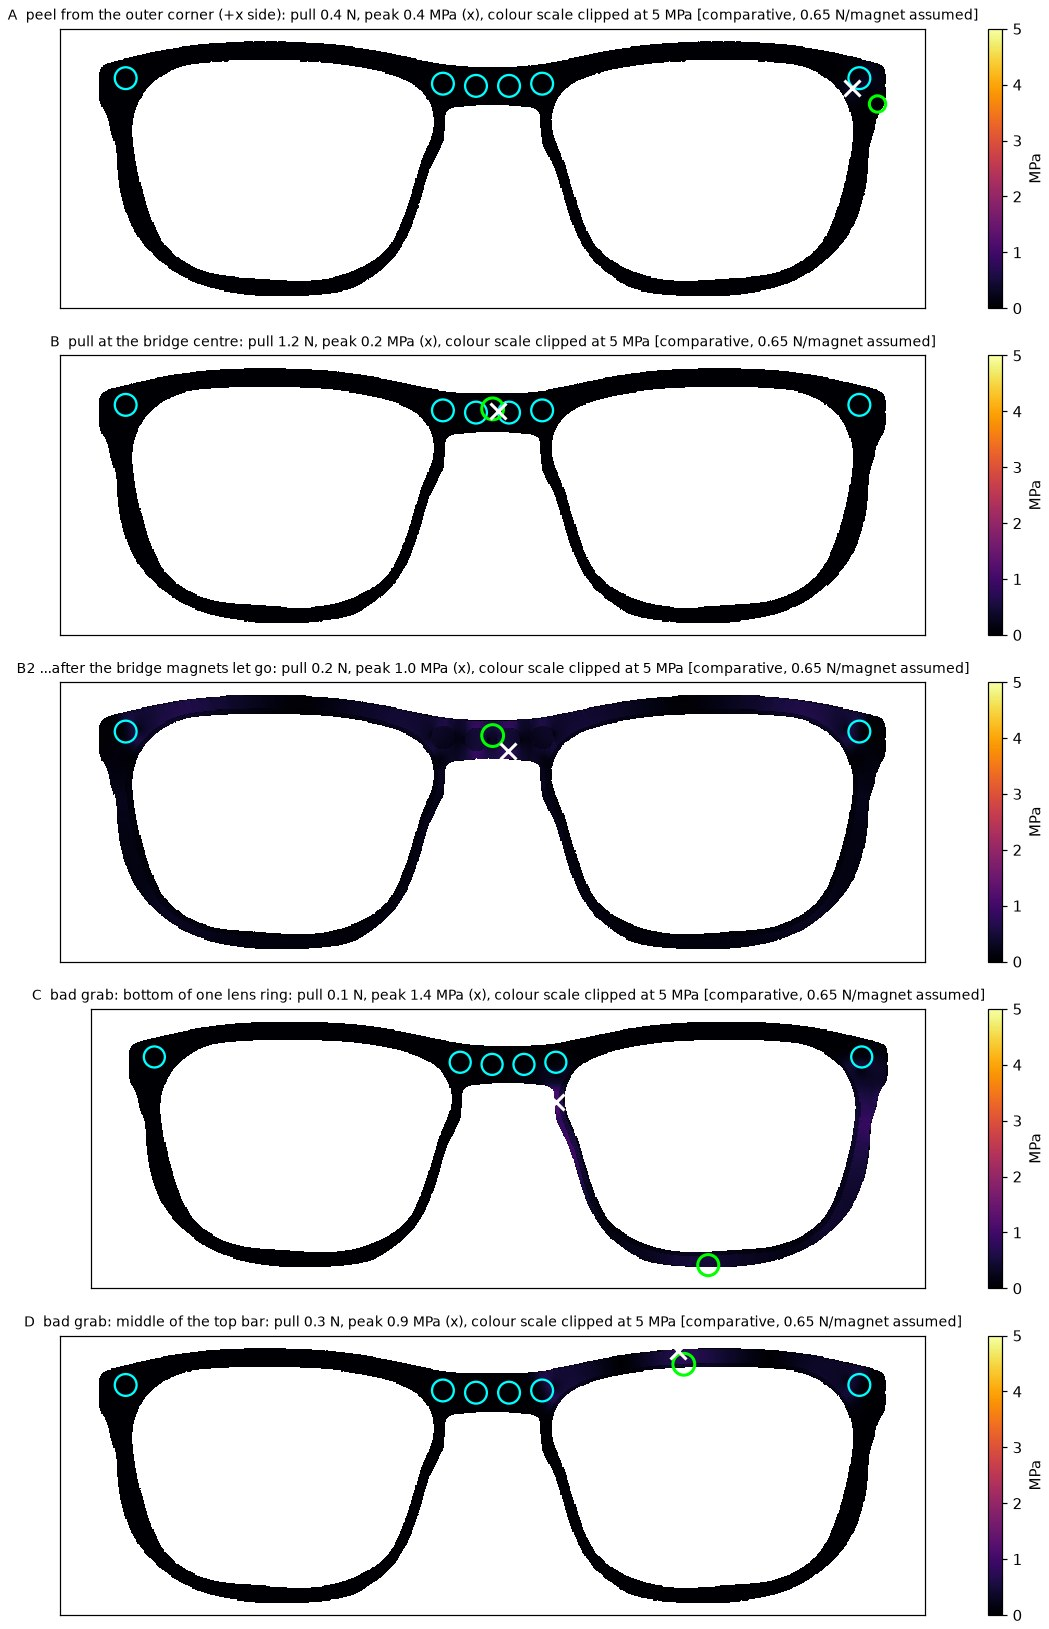
\includegraphics[height=4.82cm]{figures/stress.jpg}\hfill
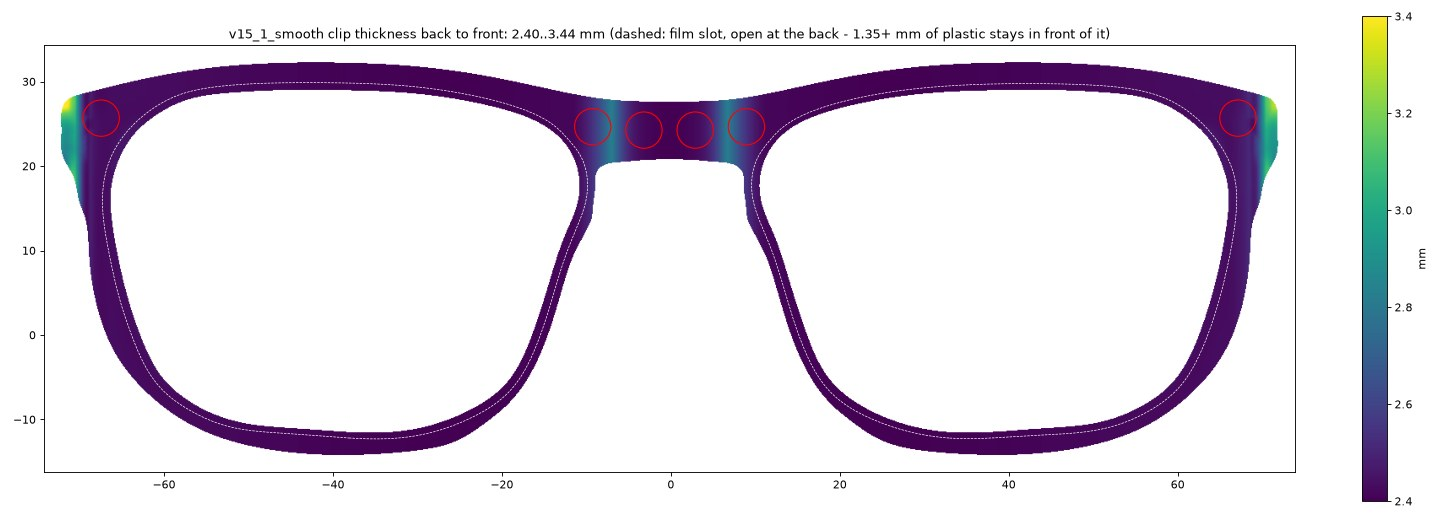
\includegraphics[height=4.82cm]{figures/thickness.jpg}
\caption{Plate-model FEA with one-way steel contact and five removal cases (peak 1.4 MPa in the worst grab), and the wall-thickness map. Comparative, not absolute.}
\end{figure}

\Needspace{12\baselineskip}\subsection{Gate 5 -- Film loading}
\begin{figure}[H]\centering
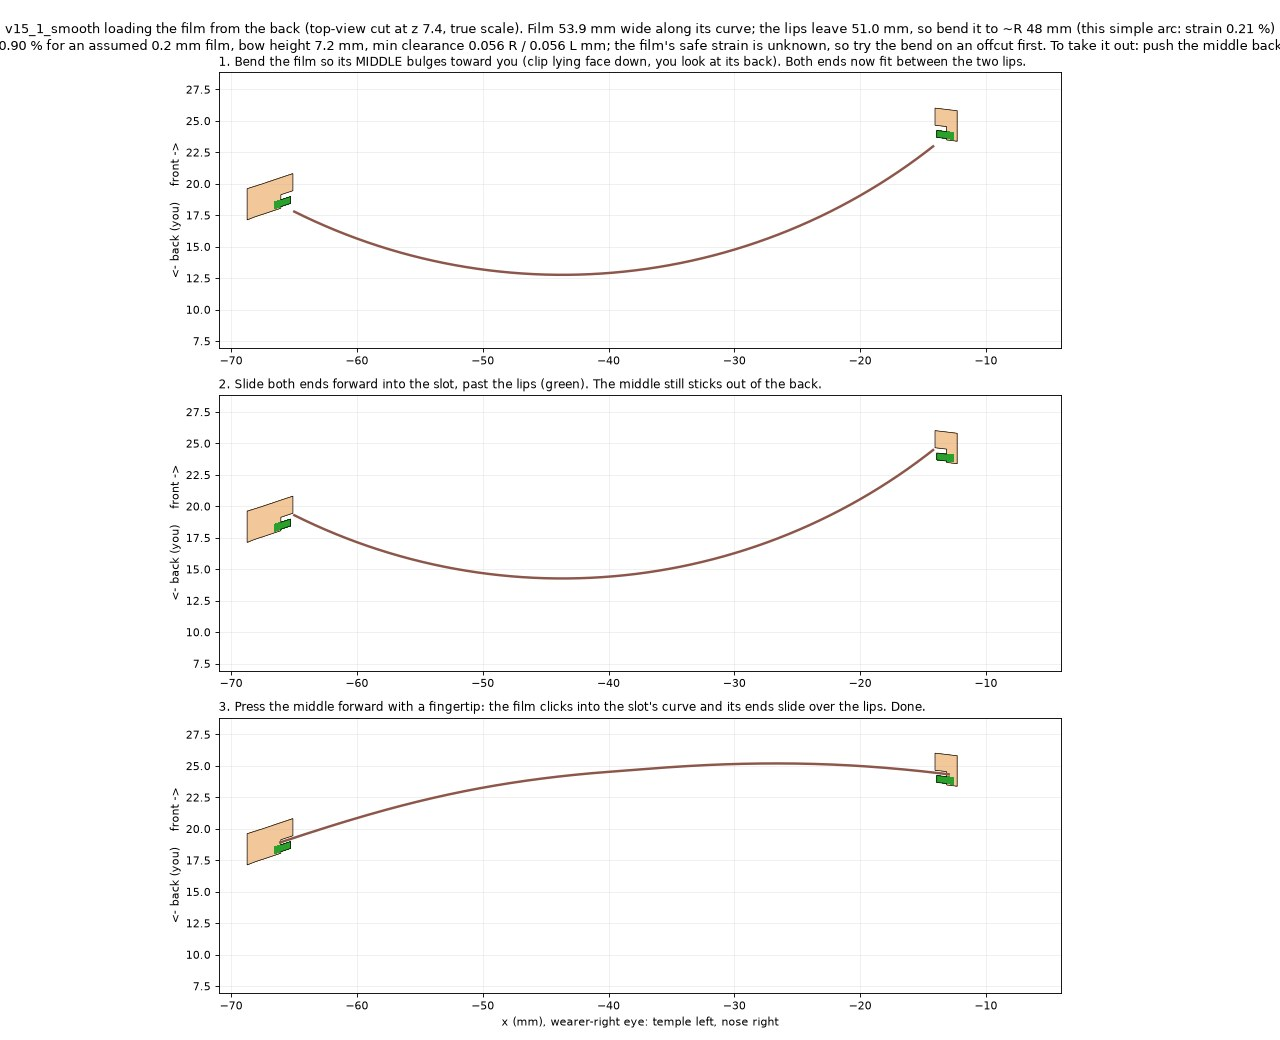
\includegraphics[height=6.59cm]{figures/film_loading.jpg}\hfill
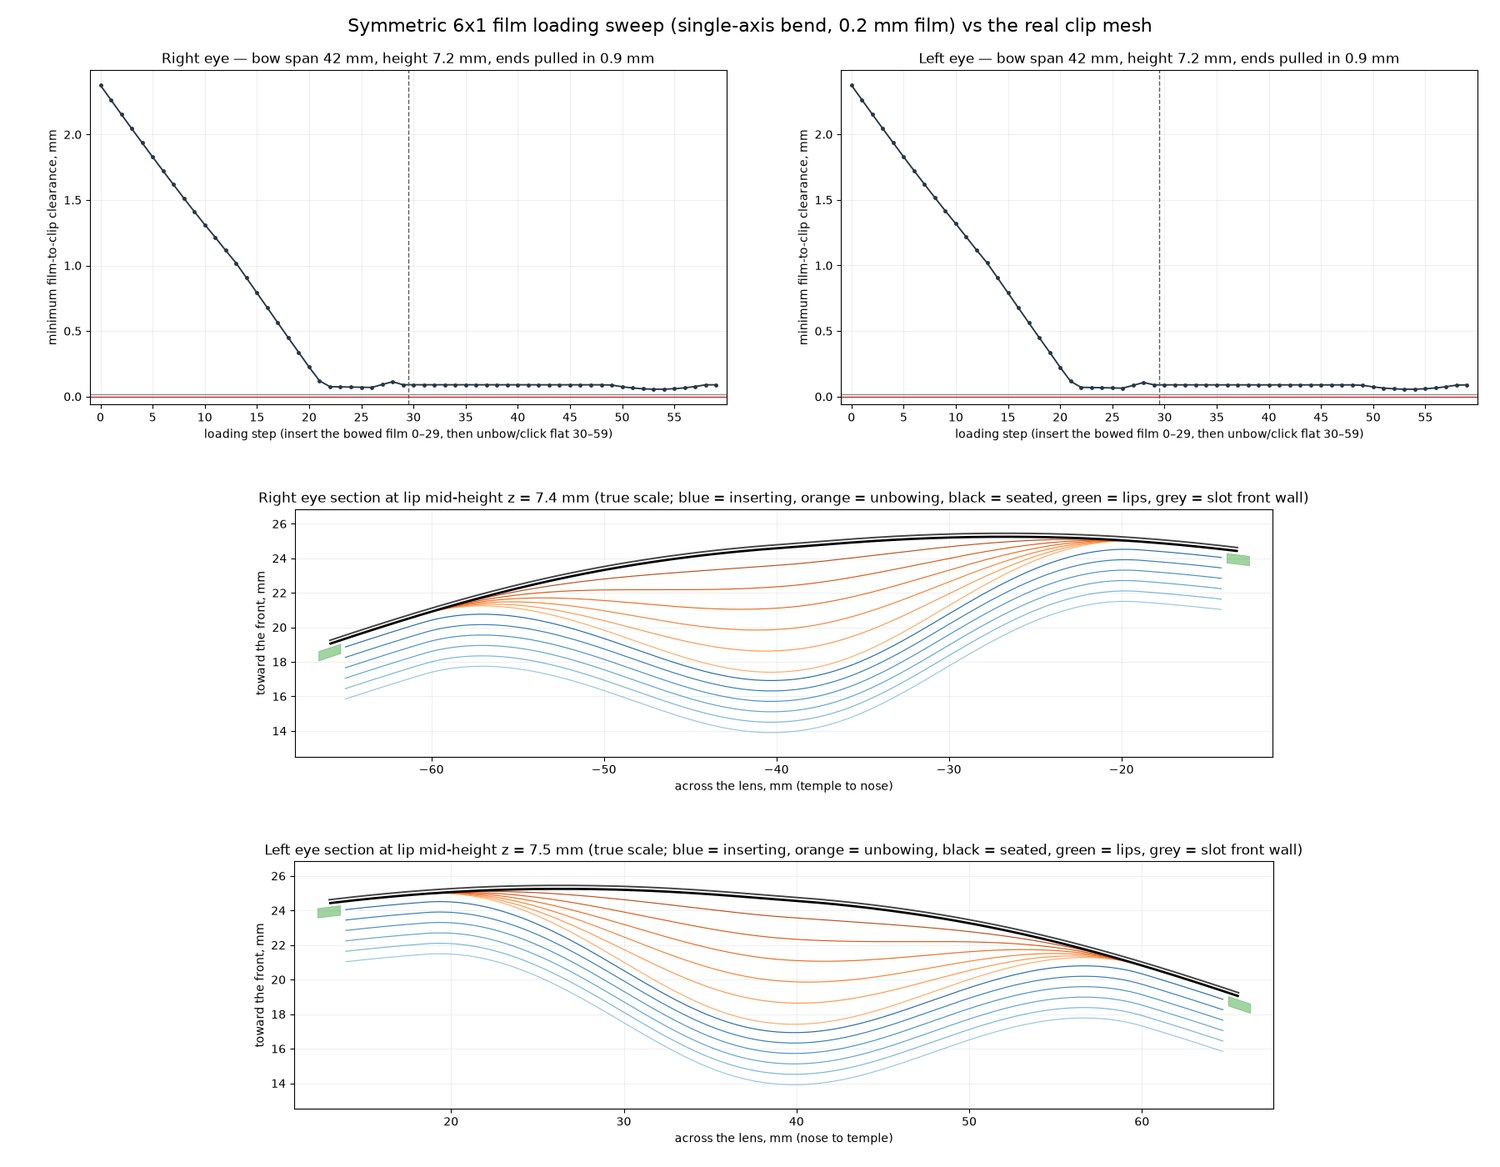
\includegraphics[height=6.59cm]{figures/loading_sweep.jpg}
\caption{The film is bowed about 7 mm in the middle, set in from the back and snaps flat. The sweep checks every intermediate state: minimum clearance 0.056 mm, peak bending strain 0.898\% against an assumed 1\% limit (the film's real limit is unknown).}
\end{figure}

\Needspace{12\baselineskip}\subsection{Gate 6 -- View and comfort}
\begin{figure}[H]\centering
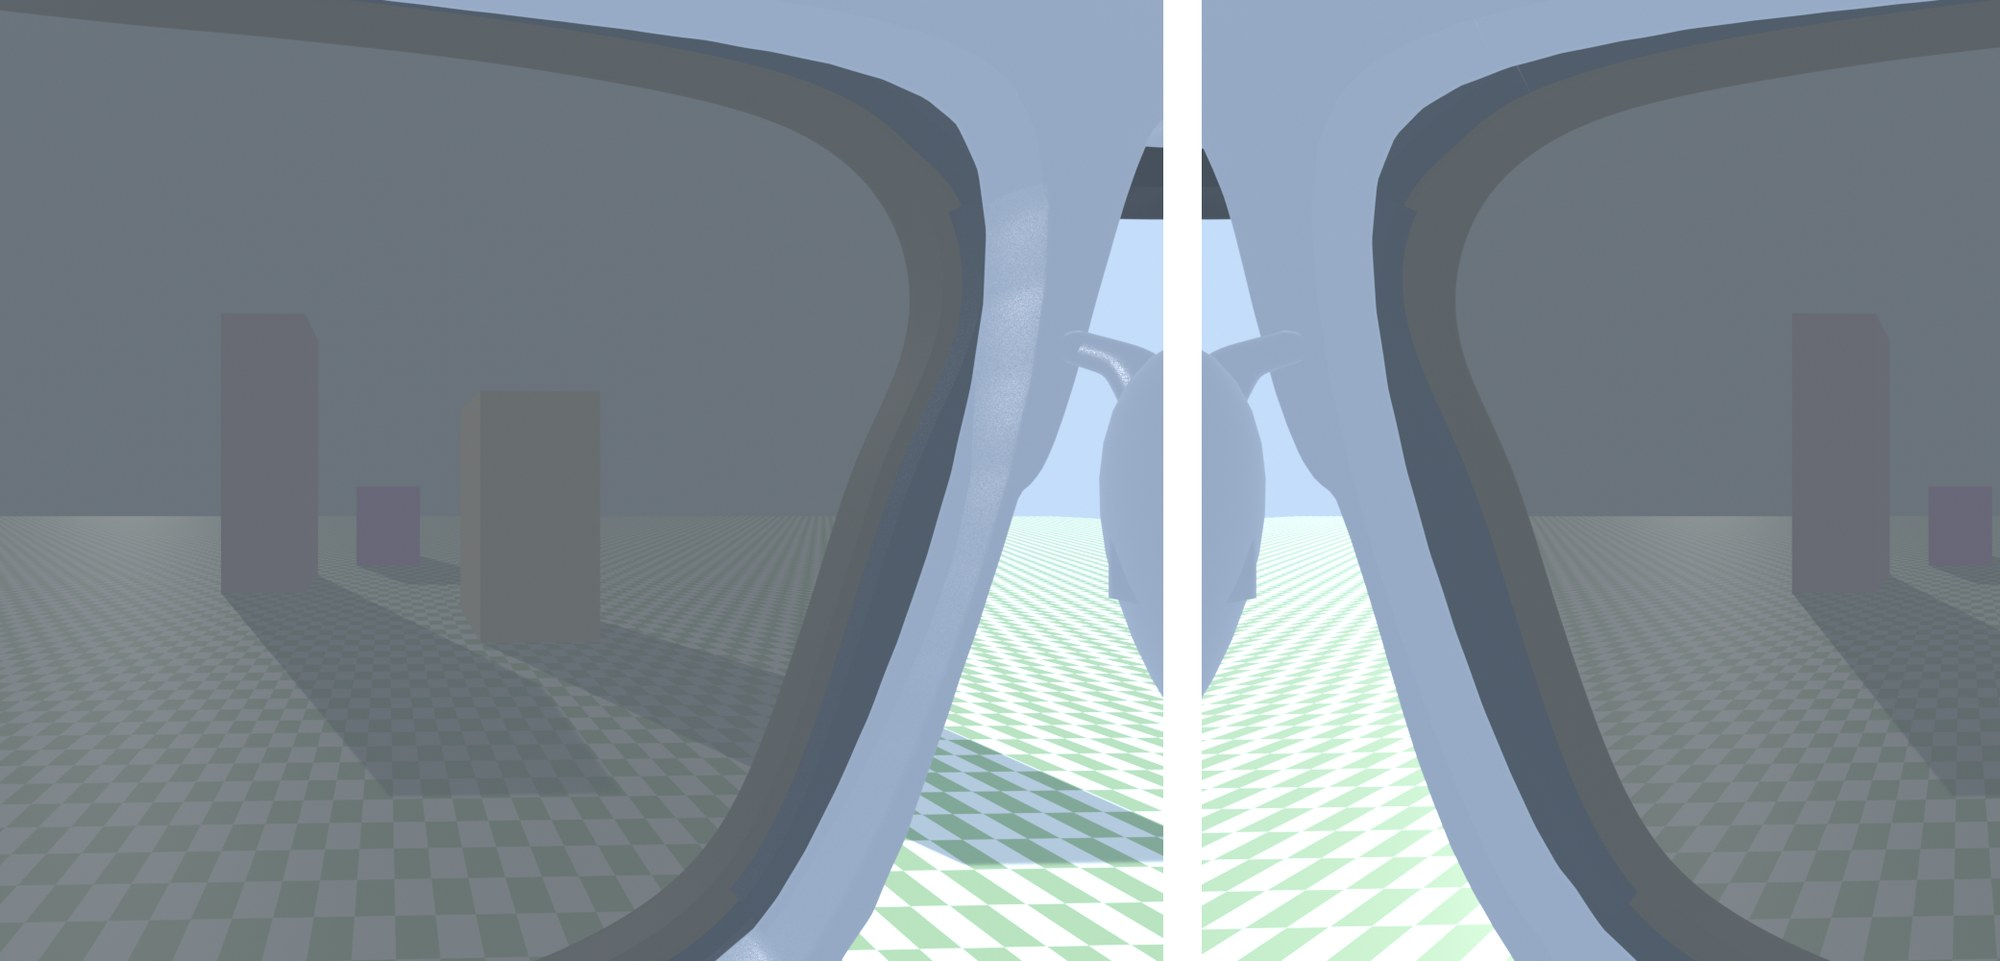
\includegraphics[height=4.69cm]{figures/eye_view.jpg}\hfill
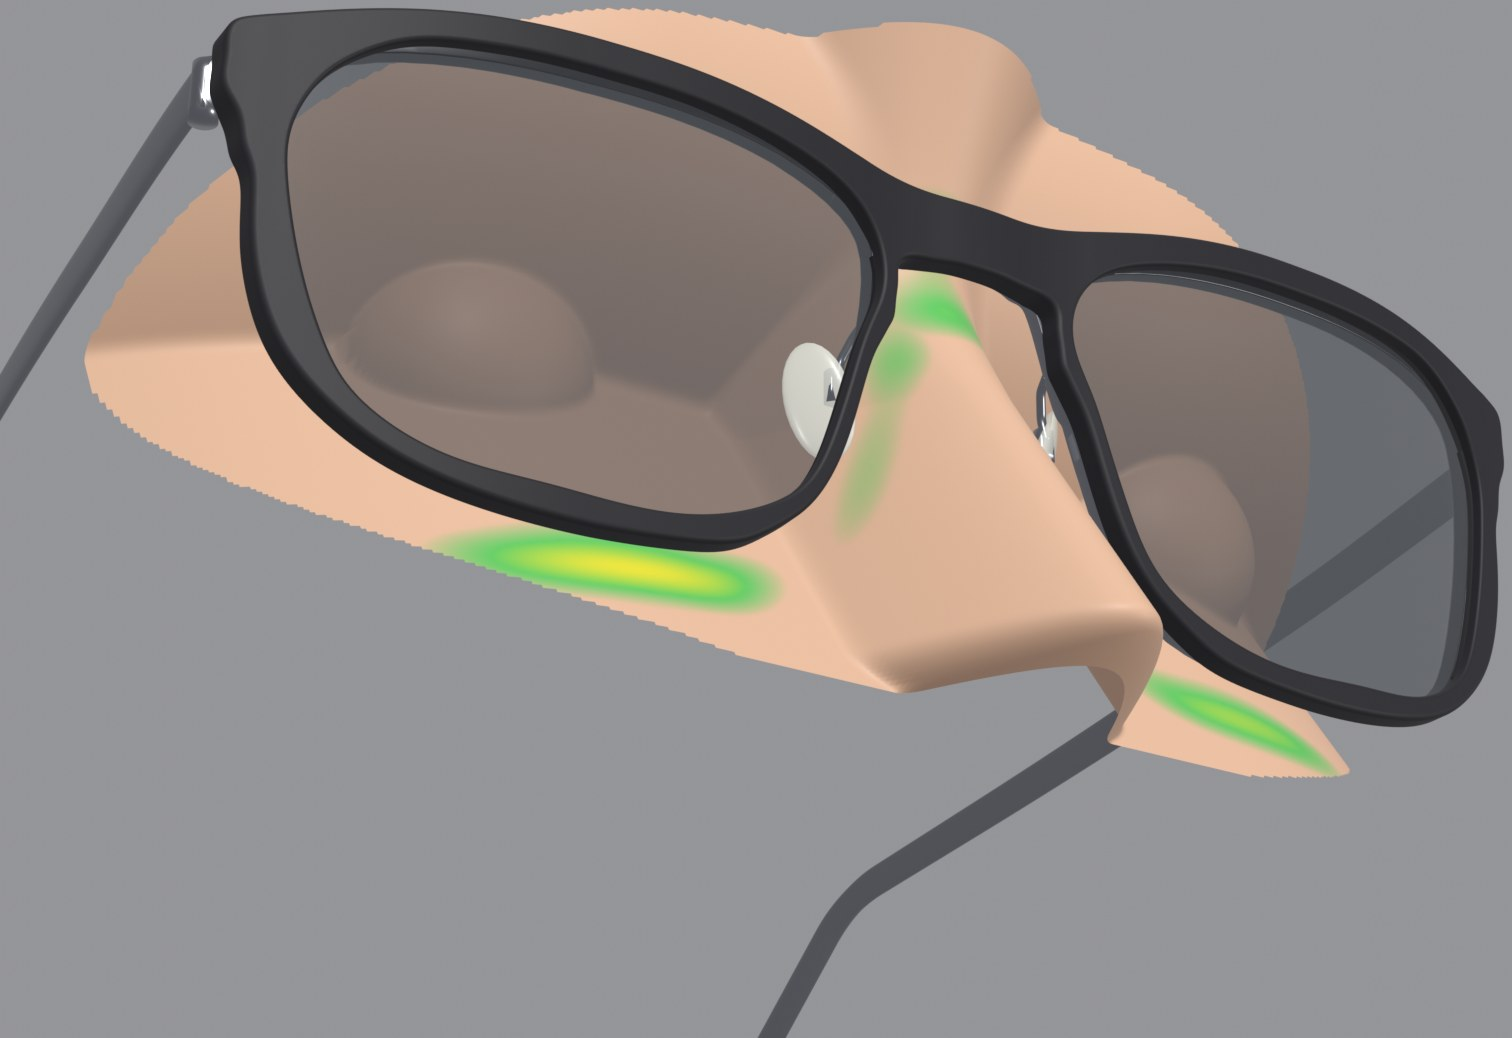
\includegraphics[height=4.69cm]{figures/face_3q.jpg}
\caption{Left: what the eye sees through both lenses. Right: a face fitted to my photo's proportions; 5,948 nose variants tested, none touch; the cheek gap below the lower rims is the one to watch (my photo itself stays private).}
\end{figure}

\Needspace{12\baselineskip}\subsection{Gate 7 -- Printability}
\begin{figure}[H]\centering
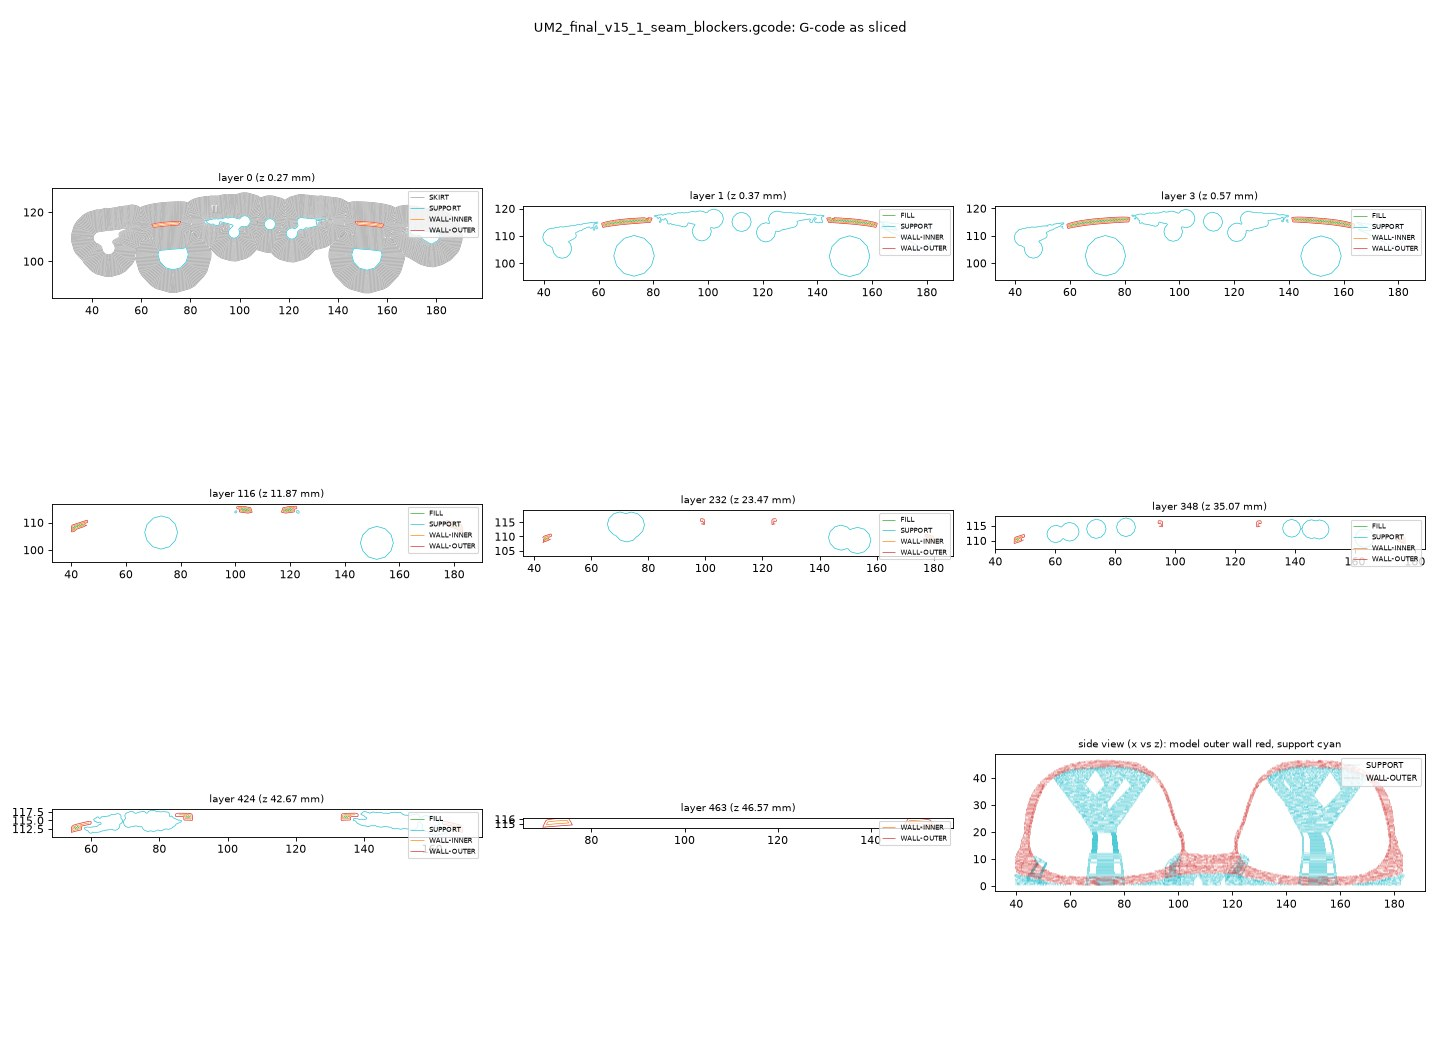
\includegraphics[width=0.9\linewidth]{figures/gcode.jpg}\\[4pt]
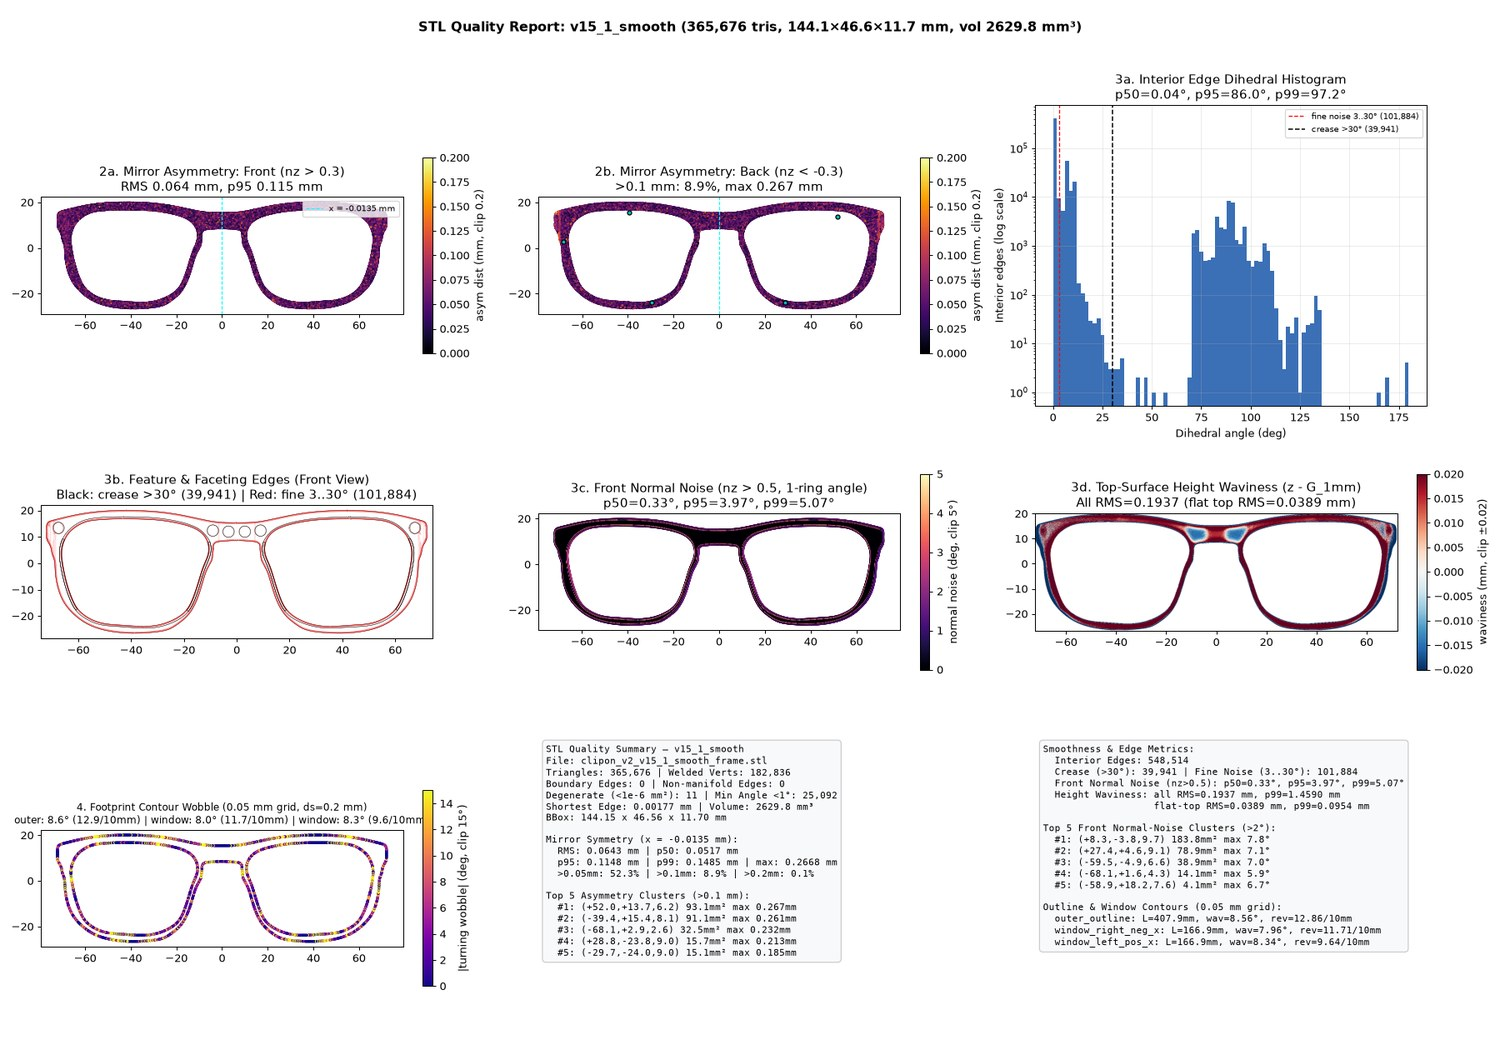
\includegraphics[width=\linewidth]{figures/stl_quality.jpg}
\caption{Top: slicer preview. Bottom: mesh checks. Printed upright (after I questioned the flat orientation), 0.1 mm layers, tree supports, blockers keep supports out of the magnet pockets. Mesh: one shell, no non-manifold edges.}
\end{figure}

\clearpage\section{The final design}
\begin{figure}[H]\centering
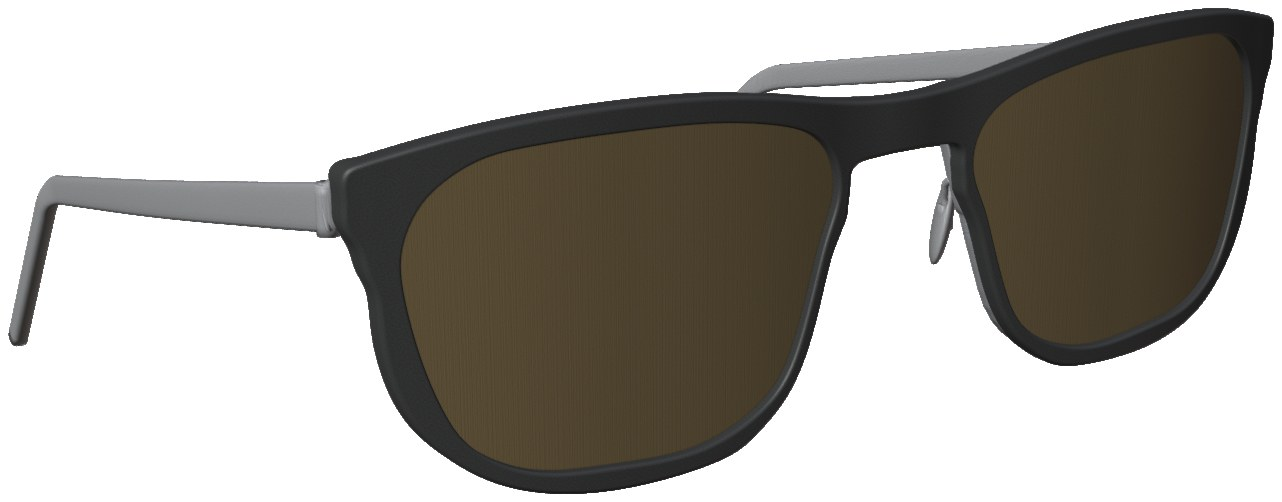
\includegraphics[width=\linewidth]{figures/render_3q.jpg}\\[4pt]
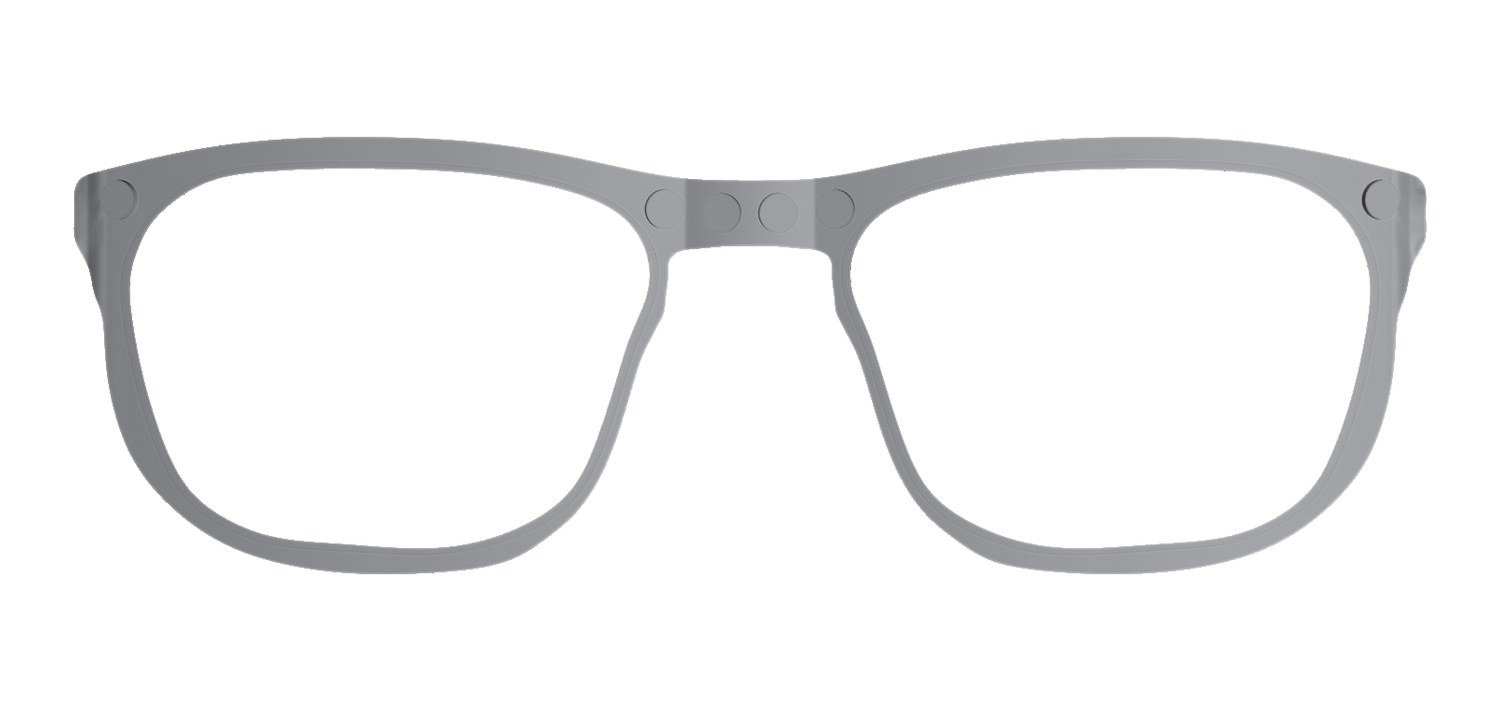
\includegraphics[width=\linewidth]{figures/render_back.jpg}\\[4pt]
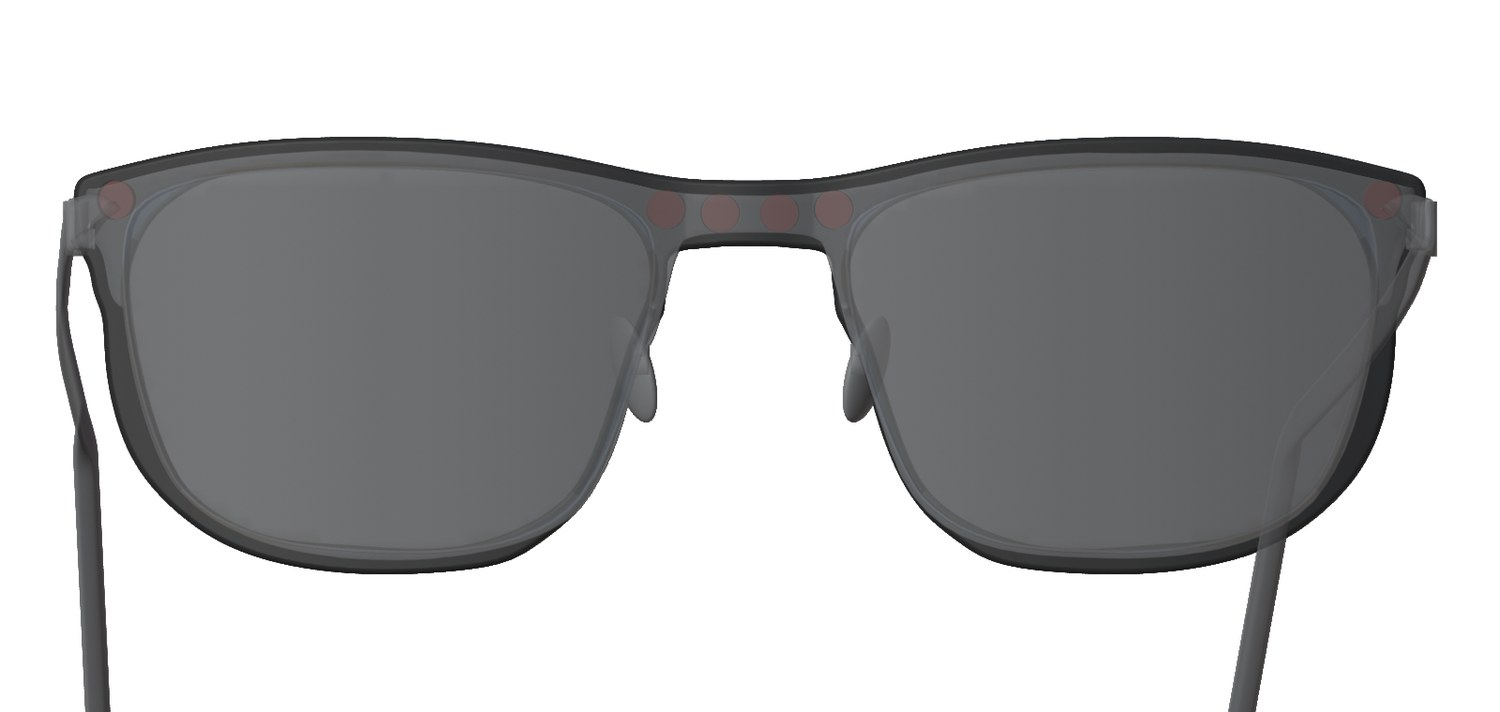
\includegraphics[width=0.495\linewidth]{figures/render_xray.jpg}\hfill
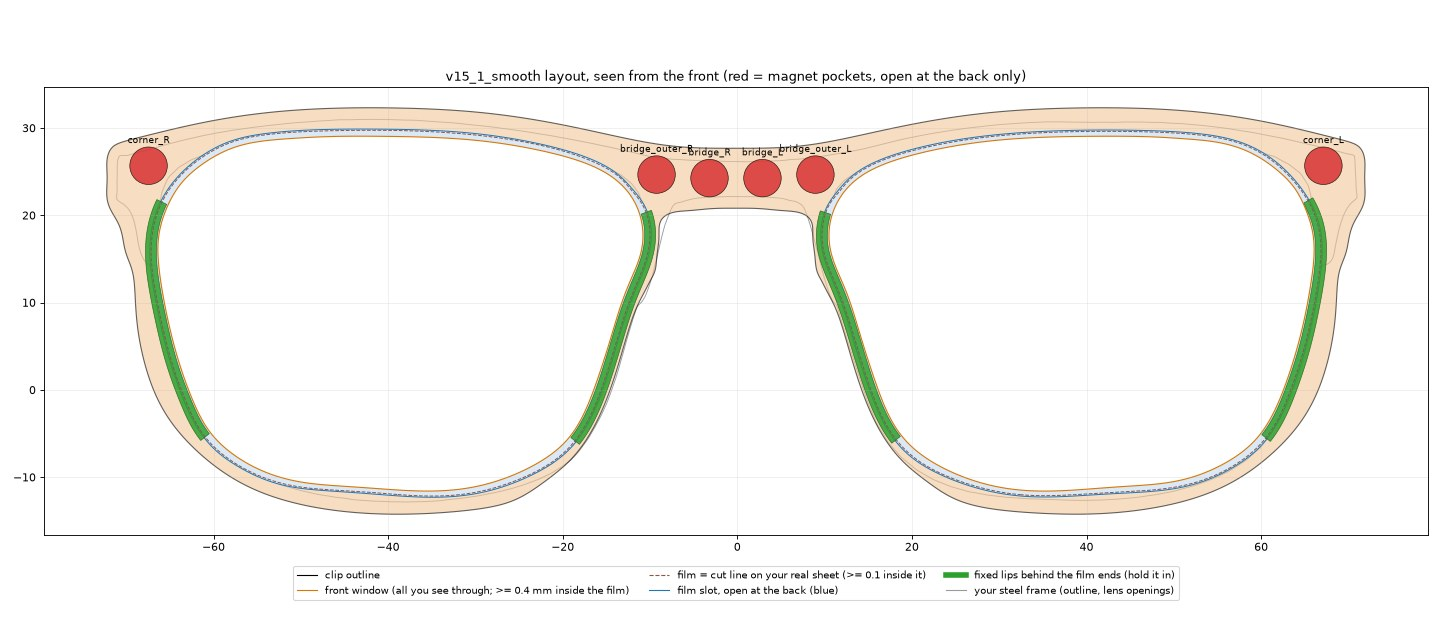
\includegraphics[width=0.495\linewidth]{figures/layout.jpg}
\caption{v15.1 on the glasses model: three-quarter view, back with the six pockets, x-ray of the film in its slot, and the design layout.}
\end{figure}

\begin{center}\small
\begin{tabularx}{\linewidth}{@{}>{\sffamily\bfseries}lX@{}}
\toprule
Clip & 144.15 mm wide, 3.26 g PLA (4.90 g with film and magnets), one piece \\
Magnets & 6 $\times$ \O4 $\times$ 1 mm NdFeB discs (172 g rated pull each), epoxied, 0.1 mm below the back surface \\
Film & 0.2 mm polarised sheets from cinema 3D glasses, loaded from the back into a 0.4 mm slot held by lips; 1:1 smooth cut template \\
View & front window leaves 97.4\% of the model lens clear (about 95.5\% of the photo-traced lens) \\
Print & Ultimaker 2+, PLA, 0.27 mm first layer then 0.1 mm, 100\% infill, 8 mm brim, tree supports, 2 h 9 min, 7.3 g with supports \\
Assembly & dry fit with loose magnets $\to$ epoxy (24 h cure) $\to$ cut film $\to$ bow-and-snap loading \\ \bottomrule
\end{tabularx}\end{center}

\begin{figure}[H]\centering
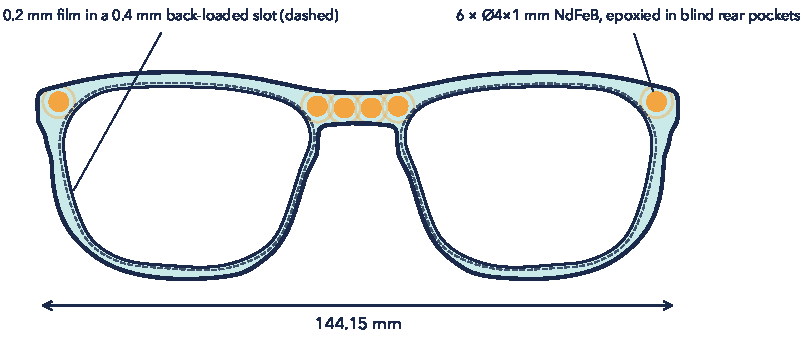
\includegraphics[width=\linewidth]{charts/blueprint.pdf}
\caption{v15.1 drawn from the design data: clip outline, front windows, film groove and the six magnet positions.}
\end{figure}

\Needspace{16\baselineskip}\section{Open items and field results}
\label{sec:field}
\begin{warnbox}
\textbf{Not verified yet.} The real pull per magnet on the thin rims; whether the front curve matches the model (the dry fit shows both); the lower-temple
corners, where photos suggest the lens edge may stand up to 0.17 mm proud of the model; the true film thickness (0.2 mm assumed).
\end{warnbox}
\begin{tcolorbox}[enhanced,colback=white,colframe=grey,boxrule=0.6pt,arc=3pt,borderline={0.6pt}{2pt}{grey,dashed},fontupper=\sffamily\small]
\faClock\enspace\textbf{Reserved: results after the print arrives.} Dry-fit photos, paper-slip test at the corners and bridge, measured pull per magnet,
first movie-night verdict, and any changes made as a result.
\end{tcolorbox}

% =====================================================================  PART II
\clearpage\part{Community playbook: build one for your glasses}

\Needspace{16\baselineskip}\section{Before you start}
\begin{keyidea}
This is the procedure I propose, not the only way. My project took 21 versions because I was discovering the problems. With the rules and prompts
below you should need far fewer. Budget a few evenings, and do not print until every check you can see passes.
\end{keyidea}

\Needspace{12\baselineskip}\subsection{Prerequisites}
\begin{center}\small
\begin{tabularx}{\linewidth}{@{}>{\sffamily\bfseries}p{2.6cm}X>{\raggedright\arraybackslash}p{3.6cm}@{}}
\toprule
 & What you need & Why \\ \midrule
Glasses & Your prescription glasses. Steel front $\to$ magnetic route; plastic, titanium or rimless $\to$ clamp route. Test with any fridge magnet. & decides the grip \\
Film & One pair of passive (polarised) cinema 3D glasses. Do not swap left and right. & the optics \\
Photos & Front, top and side photos as square-on as possible, plus the glasses on grid paper with a coin. Use a longer lens or zoom to reduce perspective. & shape and true scale \\
Outlines & Trace the front outline and the top curve yourself (Blender curve or on paper). & shape truth \\
Software & Blender (free), Python 3, an AI coding agent that can run Blender headless, a slicer (Cura). & build and check \\
Hardware & 3D printer access (0.4 mm nozzle, 0.1 mm layers), PLA or PETG; calipers or a ruler; craft knife; 2-part epoxy. & make it \\
Magnets & (magnetic route) \O4$\times$1 mm N52 discs, about 10 (6 used); 2-part epoxy only. & hold \\
Time & 3--6 evenings for the design; 2--3 h print; 24 h epoxy cure. & \\ \bottomrule
\end{tabularx}\end{center}

\Needspace{12\baselineskip}\subsection{Which route?}
\begin{center}
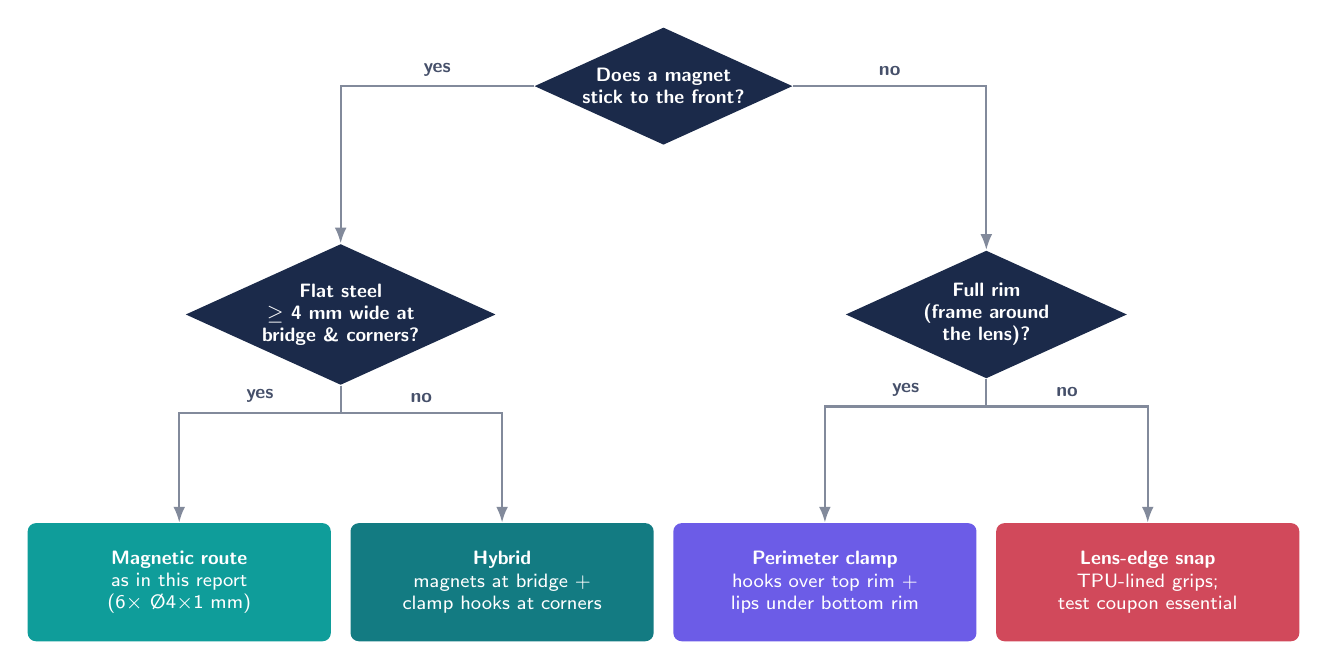
\begin{tikzpicture}[
  q/.style={diamond,aspect=2.2,fill=navy,text=white,font=\sffamily\scriptsize\bfseries,align=center,inner sep=1pt},
  r/.style={rounded corners=3pt,fill=#1,text=white,font=\sffamily\scriptsize,align=center,minimum width=3.85cm,minimum height=15mm,text width=3.6cm},
  ar/.style={-{Latex[length=2mm]},line width=0.8pt,navy!55},lab/.style={font=\sffamily\scriptsize\bfseries,text=slate}]
  \node[q] (q1) at (0,0) {Does a magnet\\stick to the front?};
  \node[q] (q2) at (-4.1,-2.9) {Flat steel\\$\ge$ 4 mm wide at\\bridge \& corners?};
  \node[q] (q3) at (4.1,-2.9) {Full rim\\(frame around\\the lens)?};
  \node[r=teal] (m1) at (-6.15,-6.3) {\textbf{Magnetic route}\\as in this report\\(6$\times$ \O4$\times$1 mm)};
  \node[r=teal!70!navy] (m2) at (-2.05,-6.3) {\textbf{Hybrid}\\magnets at bridge +\\clamp hooks at corners};
  \node[r=violet] (c1) at (2.05,-6.3) {\textbf{Perimeter clamp}\\hooks over top rim +\\lips under bottom rim};
  \node[r=coral] (c2) at (6.15,-6.3) {\textbf{Lens-edge snap}\\TPU-lined grips;\\test coupon essential};
  \draw[ar] (q1) -| node[lab,above,pos=0.25]{yes} (q2); \draw[ar] (q1) -| node[lab,above,pos=0.25]{no} (q3);
  \draw[ar] (q2.south) -- ++(0,-0.35) -| node[lab,above,pos=0.25]{yes} (m1); \draw[ar] (q2.south) -- ++(0,-0.35) -| node[lab,above,pos=0.25]{no} (m2);
  \draw[ar] (q3.south) -- ++(0,-0.35) -| node[lab,above,pos=0.25]{yes} (c1); \draw[ar] (q3.south) -- ++(0,-0.35) -| node[lab,above,pos=0.25]{no} (c2);
\end{tikzpicture}
\end{center}

\Needspace{16\baselineskip}\section{The procedure in ten steps}
\begin{center}
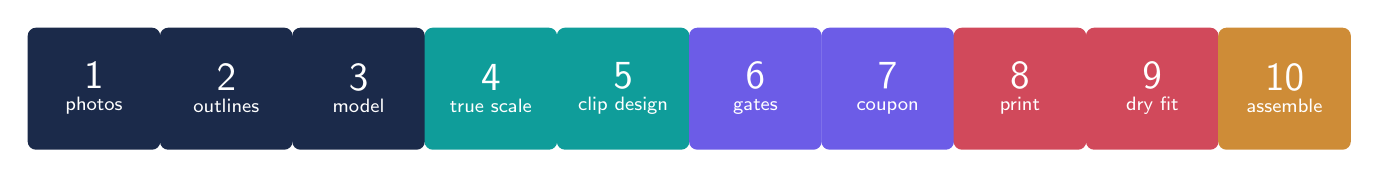
\begin{tikzpicture}[s/.style={rounded corners=3pt,fill=#1,text=white,minimum width=1.55cm,minimum height=1.55cm,font=\sffamily\scriptsize,align=center,text width=1.45cm}]
\foreach \i/\t/\c in {1/photos/navy,2/outlines/navy,3/model/navy,4/true scale/teal,5/clip design/teal,6/gates/violet,7/coupon/violet,8/print/coral,9/dry fit/coral,10/assemble/amber!85!black}
  \node[s=\c] at ({(\i-1)*1.68},0) {{\heavy\Large \i}\\\t};
\end{tikzpicture}
\end{center}
\begin{enumerate}[leftmargin=18pt,label=\textbf{\sffamily\color{teal}\arabic*.}]
\item \textbf{Photograph} the glasses front, top and side, square on, on a plain background; then on grid paper with a known coin.
\item \textbf{Trace the outlines yourself}: front outline and top curve. Declare them the only source of shape.
\item \textbf{Build the glasses model} from the photos on three axes. Ask for overlays and an alignment number; allow 1--2$^\circ$ photo tilt correction. Make it mirror-symmetric if your frame is.
\item \textbf{Prove the true scale} from at least two independent sources (grid, coin, the size printed on the temple, e.g. 57\,\fbox{\rule{0pt}{1ex}}\,20-145). Do not continue until they agree.
\item \textbf{Design the clip}: outline flush with the frame, film slot from the back, magnet pockets square to the steel (or clamp hooks), smooth curves only.
\item \textbf{Run the gates}: shape, contact gap, magnet seating, strength, film loading, view, face comfort, printability. Ask for the plots, not a summary.
\item \textbf{Print a test coupon} of the bridge and one corner first (minutes of print time) and try it on the real glasses.
\item \textbf{Print} upright with supports kept out of the pockets; 0.1 mm layers.
\item \textbf{Dry fit} with loose magnets: no rocking; printer paper must not slide under the magnet spots.
\item \textbf{Assemble}: epoxy the magnets (never super glue), cure 24 h, cut the film with the 1:1 template, bow and snap it in from the back.
\end{enumerate}

\Needspace{16\baselineskip}\section{Prompt pack}
These are distilled from my own prompts. Replace \texttt{<...>}. The full set, including the non-metal clamp prompts, is in \texttt{prompts/PROMPT\_PLAYBOOK.md}.

\begin{template}{P1 \textbullet{} Set the rules first (send once, at the start)}
I am designing a 3D-printed clip-on that holds flat polarised 3D-cinema film in front of my prescription glasses (<frame type>).
Rules for the whole project: (1) Shape comes ONLY from my hand-drawn outlines <files>; photos set size, never shape. (2) Never modify my
original objects or files; build each version in its own folder with a report. (3) I have one chance to print: never present a design with
a defect your own analysis shows. (4) Every claim needs evidence: a number, a plot or a section view. (5) The film can bend in one direction,
never dome. (6) No CA/super glue near the film.
\end{template}

\begin{template}{P2 \textbullet{} Build the glasses model from photos}
Open <file>.blend. It has three reference photos (front, top, side) and my outlines. Build my glasses in 3D from the photos on all three
axes, not from any scan. My photos may be 1-2 degrees off square; you may rotate the images to align. Show overlays of the model on each photo
and report the alignment error in mm. The front must be exact because I will attach to it.
\end{template}

\begin{template}{P3 \textbullet{} Prove the true scale}
Here are photos of my glasses on <6 mm> grid paper with a <coin name> and the temple marking <57[]20-145>. Look up the coin's exact diameter.
Measure the model's scale from each source separately, show the overlays, and tell me whether they agree. If one source disagrees,
show me why before choosing. I want precision like 2.345 mm, not "about right".
\end{template}

\begin{template}{P4 \textbullet{} Magnet layout I can judge myself}
I have <N> magnets of <4 x 1 mm, rated pull 172 g on 10 mm steel>. Account for vertical mounting, thin steel and air gap.
Show a front view of the frame with a colour gradient for depth and flatness, and mark where a magnet keeps full contact.
Show me where you place each magnet; I will mark where I would put them and you explain why not.
\end{template}

\begin{template}{P5 \textbullet{} Independent review with lenses}
Give the model, my full request history and the rules to <2-3> other models. Each reviews through one lens: (a) making and using
the real part, (b) smoothness and print quality, (c) accuracy against my outlines. Findings must cite a number, a file line or a
render region. Verify each finding yourself; change the design only if it is real and serves my goal.
\end{template}

\begin{template}{P6 \textbullet{} Final audit before printing}
Before I print: list every check (fit, contact, magnets, strength, film loading, view, comfort, printability, size) with the
number, the threshold and the plot. List what is NOT verified. Do not say ready unless every visible issue is fixed.
\end{template}

\Needspace{16\baselineskip}\section{If your frame is not magnetic: clamp from all sides}
Plastic (acetate), titanium and many alloy frames do not attract magnets. The same pipeline works; only the grip changes.
My recommendation is a \textbf{perimeter clamp}: small hooks over the top rim and lips under the bottom rim on both lenses, so the clip grips the
frame from all sides at once. The load is shared by many small contacts, there is no single pressure point, and the clip self-centres.

\begin{center}
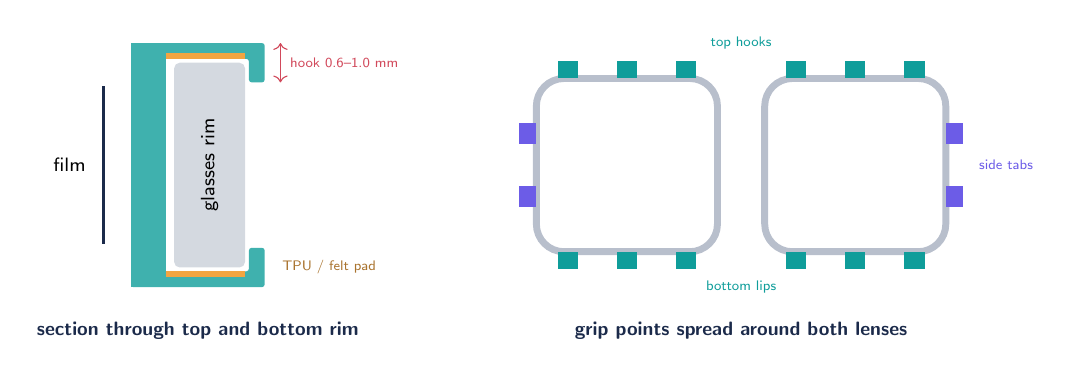
\begin{tikzpicture}[scale=1.0]
  % section through a rim with the clamp
  \begin{scope}
    \fill[grey!60,rounded corners=2pt] (0,0) rectangle (0.9,2.6);
    \node[font=\sffamily\scriptsize,rotate=90] at (0.45,1.3) {glasses rim};
    \fill[teal!80] (-0.55,-0.25) rectangle (-0.1,2.85);
    \fill[teal!80,rounded corners=1pt] (-0.55,2.85) -- (1.15,2.85) -- (1.15,2.35) -- (0.95,2.35) -- (0.95,2.65) -- (-0.1,2.65) -- cycle;
    \fill[teal!80,rounded corners=1pt] (-0.55,-0.25) -- (1.15,-0.25) -- (1.15,0.25) -- (0.95,0.25) -- (0.95,-0.05) -- (-0.1,-0.05) -- cycle;
    \fill[amber] (-0.1,2.65) rectangle (0.9,2.72); \fill[amber] (-0.1,-0.12) rectangle (0.9,-0.05);
    \draw[navy,line width=1.2pt] (-0.9,0.3) -- (-0.9,2.3); \node[font=\sffamily\scriptsize,anchor=east] at (-1.0,1.3) {film};
    \draw[<->,coral] (1.35,2.35) -- node[right,font=\sffamily\tiny]{hook 0.6--1.0 mm} (1.35,2.85);
    \node[font=\sffamily\tiny,text=amber!70!black,anchor=west] at (1.25,0.0) {TPU / felt pad};
    \node[font=\sffamily\scriptsize\bfseries,text=navy] at (0.3,-0.8) {section through top and bottom rim};
  \end{scope}
  \begin{scope}[xshift=7.2cm,yshift=1.3cm]
    \draw[grey,line width=2.5pt,rounded corners=10pt] (-2.6,1.1) rectangle (-0.3,-1.1);
    \draw[grey,line width=2.5pt,rounded corners=10pt] (0.3,1.1) rectangle (2.6,-1.1);
    \foreach \x in {-2.2,-1.45,-0.7,0.7,1.45,2.2} {\fill[teal] (\x-0.13,1.1) rectangle (\x+0.13,1.32); \fill[teal] (\x-0.13,-1.1) rectangle (\x+0.13,-1.32);}
    \foreach \y in {-0.4,0.4} {\fill[violet] (-2.82,\y-0.13) rectangle (-2.6,\y+0.13); \fill[violet] (2.6,\y-0.13) rectangle (2.82,\y+0.13);}
    \node[font=\sffamily\scriptsize\bfseries,text=navy] at (0,-2.1) {grip points spread around both lenses};
    \node[font=\sffamily\tiny,text=teal] at (0,1.55) {top hooks};
    \node[font=\sffamily\tiny,text=teal] at (0,-1.55) {bottom lips};
    \node[font=\sffamily\tiny,text=violet,anchor=west] at (2.9,0) {side tabs};
  \end{scope}
\end{tikzpicture}
\end{center}
\begin{itemize}
\item Clearance: start at 0.15--0.3 mm per side and tune it with a printed coupon of one corner; plastic frames vary.
\item Hooks: 0.6--1.0 mm deep, filleted at the root; print so layer lines run \emph{across} the hook, not along it, or it will snap.
\item Never press on the lens face or its coating; line contact points with thin TPU or felt.
\item Keep clear of nose pads, hinges and the field of view; the gates (view, comfort) still apply.
\item Full comparison of grip options, rules, prompts and checklists: \texttt{guide/NON\_METAL\_FRAMES.md}.
\end{itemize}

\Needspace{16\baselineskip}\section{Lessons for the community}
\begin{multicols}{2}\small
\textbf{\sffamily\color{teal}1. The model is the foundation.} A third of my prompts went into the glasses model. Every later error (gaps, spikes, scale) traced back to it.

\textbf{\sffamily\color{teal}2. AI confidence is not evidence.} ``Ready to print'' was said several times before it was true. Ask for the plot.

\textbf{\sffamily\color{teal}3. Read the datasheet yourself.} Rated magnet pull assumes thick horizontal steel; on a thin vertical rim expect a fraction of it.

\textbf{\sffamily\color{teal}4. Your own photos are measuring instruments.} Grid paper and a well-known coin beat any assumption about size.

\textbf{\sffamily\color{teal}5. Do not let photo noise into cut lines.} Traced outlines wiggle; anything you cut by hand should be a smooth curve.

\textbf{\sffamily\color{teal}6. Keep every version.} A rejected variant is the proof of why the final one is right (v16 and v18 saved me from two wrong prints).

\textbf{\sffamily\color{teal}7. Print a coupon.} A bridge-and-corner coupon costs minutes and catches what no simulation can.

\textbf{\sffamily\color{coral}8. Safety.} Never super glue near the film; never walk around or drive wearing 3D film; stop if it presses on your nose or cheeks.
\end{multicols}

\appendix
\Needspace{16\baselineskip}\section{Version ledger}
\small
\begin{tabularx}{\linewidth}{@{}>{\sffamily\bfseries}p{1.1cm}>{\raggedright\arraybackslash}p{5.6cm}>{\raggedright\arraybackslash}X>{\sffamily\scriptsize}p{1.9cm}@{}}
\toprule
Ver. & Idea & Why it was replaced & Status \\ \midrule
v00 & glasses model from photos + outlines & refined $\to$ aligned $\to$ symmetric $\to$ $\times$1.011 & base \\
v01 & first clip, film uncut & film too big, protruded & superseded \\
v02 & film cut to lens outline & protruded towards the nose & superseded \\
v03 & clip never past the steel & magnets not chosen yet & superseded \\
v04 & flush, 4$\times$1 mm magnets & cut too much film & superseded \\
v05 & wide clip, film almost uncut & border too weak & superseded \\
v06 & wider plastic border & magnet padding & superseded \\
v07 & magnets at my sketched spots & model drift found (two spikes) & superseded \\
v08 & first clip on the aligned model & visible gap, slanted holes & superseded \\
v09 & square pockets, smooth front & film loading method & superseded \\
v10 & film slot open at the back & film shape from real sheets & superseded \\
vX & ChatGPT/Codex side attempt & fictional film contour & rejected \\
v11 & film cut from the two real sheets & asymmetric, hold under-estimated & superseded \\
v12 & mirror-symmetric, 4 magnets & four magnets judged too few & superseded \\
v13 & six single magnets & bridge underside, review findings & superseded \\
v14 & faired bridge arch, comfort checks & size never proven & superseded \\
v15 & rebuilt at measured $\times$1.011 & wiggly film slot and cut & superseded \\
v16 & reshaped to a photo re-trace & broke the outline rule & rejected \\
v17 & film slot from photo re-trace & abandoned with v16 & abandoned \\
v18 & height $\times$1.026 & 1.3\% too tall vs 3 of 4 sources & kept \\
\rowcolor{teal!10} v15.1 & smooth slot, lips and cut & -- & \textbf{FINAL} \\ \bottomrule
\end{tabularx}
\normalsize

\Needspace{16\baselineskip}\section{Reproducing the figures}
\raggedright
Figures come from the private design workspace (Blender scenes and analysis scripts). \texttt{scripts/collect\_figures.py} copies them,
\texttt{scripts/make\_charts.py} draws the charts, and \texttt{scripts/curate\_prompts.py} produces the curated prompt log.
Build this report with \texttt{xelatex main.tex} (twice).
\end{document}
